% !Mode:: "TeX:UTF-8"
\chapter{国内外研究现状}\label{chap:related_work}

本章旨在综述国内外关于本文研究内容的相关工作。首先,本章将介绍当前计算机视觉领域中与分类和检测任务相关的神经网络模型。特别地将重点介绍并分析分类任务中的CNN系列、Transformer系列和RNN系列模型和在检测任务中的U-Net系列目标分割模型、R-CNN和YOLO系列目标检测模型。其次,本章将详细介绍医学影像领域中分类任务与检测任务的最新研究进展,并对本文所涉及的假体关节感染和骨折相关感染诊断任务的特殊性和现有方法进行深入阐述。

\section{图像分类}

分类任务是指输入数据经过模型计算后分为不同的类别或者标签的任务,这是深度学习中最常见和最基本的问题之一。其中,模型需要从训练数据集中学习数据特征与标签之间的关系,用以对未见过的数据正确地从已知的多个标签集合中选择最合适的一个或几个标签。在计算机视觉领域中,对图像、视频或其他视觉数据的特征提取一直以来都是研究的核心问题。赋予计算机类似于人类一样的智慧视觉能力是多年来许多研究人员共同追求的目标和努力方向。随着相关技术的不断发展,尤其是图像识别技术的不断进步,在计算机视觉领域之中的分类任务在医疗、航海、交通等多个现实场景中有着诸多良好的应用前景,包括人脸识别、航空遥感和医学影像等等。

通常情况下,分类任务的主要流程包括特征提取和模型设计两个关键步骤。合适的特征提取和模型设计可以相辅相成,以实现较优异的性能表现。在早期,图像识别技术\cite{fu1976pattern}主要采用了基于先验知识设计的手工特征。原理在于对于不同的应用场景,需要由相应领域的专家提供专业知识去设计所需要的特征。然而,这种针对某一的领域特性和相应的数据类型进行的手工编码,难以去处理海量的数据,效率及其低下\cite{季长清2022基于卷积神经网络的图像分类算法综述}。此外,人工设计的特征的普遍性不强,图像中可能存在噪声,难以涵盖所有情形,很可能导致分类的结果并不理想。而在图像领域中,常见的形状、纹理、颜色等浅层视觉特征和局部二值模式、方向梯度直方图等局部不变特征,虽然具有一定的普适性,但应用到现实场景具体图像时,针对性不足,尤其是面对一些存在复杂场景的情形,更加难以去准确使用手工特征去描述目标图像\cite{杨真真2018基于卷积神经网络的图像分类算法综述}。

在模型方面,传统的机器学习模型实现简单,决策依据直观可理解,但对于复杂图像如图像噪声干扰较多,不同类别之间差异小等问题,其性能会大大下降。此外,传统机器学习依赖于特征提取,难以实现全自动化,性能极大受限于手工特征的有效性。随着计算机硬件的快速发展,特别是图形处理器(Graphics Processing Unit,GPU),以及大规模训练数据集(ImageNet\cite{deng2009imagenet}、CelebA\cite{liu2018large}等)的出现,深度学习方法在计算机视觉领域中其优越性在不断凸显。相比较于传统的图像识别技术,深度学习方法不再需要人工设计的手工特征,而是通过神经网络模型自主地在训练数据集中学习到潜在有效的特征,这很好地将特征提取融合到模型设计之中,解决了人工设计特征的难题。由此,深度学习方法开始逐步替代传统的机器学习方法成为了主流,得到了飞跃式的进展。

\textbf{本文围绕动态骨显像和PET/CT进行相关研究。由于动态骨显像和PET/CT的特点,导致难以直接应用深度学习方法进行影像特征提取。例如,动态骨显像和PET/CT都是单通道的图像数据,以强度的大小与分布来进行表示。其中,动态骨显像与PET可以展示人体组织生理代谢的强弱,而CT可以展示人体组织的解剖结构信息。影像中的无关区域与干扰区域会影响最终分类的精度,且单独的图像特征并不充足。动态骨显像还具有时序上的特征;而PET/CT还具有更全面的立体特征。}

\subsection{图像分类算法}

常见的机器学习模型有K-近邻算法,决策树、支持向量机等等。K-近邻算法(K-Nearest Neighbor,KNN)\cite{guo2003knn}基于一个简单的假设:相似的样本具有相似的标签。该算法通过计算样本之间的距离来代表样本之间的相似性,在训练数据集中根据每个未知样本最相似的K个邻居来对该未知样本进行分类。该算法简单直观易于理解,但计算和内存的开销大且对不平衡数据集不友好。决策树\cite{suthaharan2016decision}的基本思想是通过一系列的对某一特征值的条件筛选来对数据进行划分,直至划分到叶子结点得到最终的预测结果。该算法易于理解和解释,具有可视性,但容易过拟合和达到局部最优解。支持向量机(Support Vector Machine,SVM)\cite{suthaharan2016support}的基本思想是寻找一个可以将不同类别样本隔开的超平面,并且最大化样本与超平面之间的最小距离。该算法具有较强的泛化能力和对噪声的鲁棒性,但仅适用于二分类问题,且计算和内存的开销大。

\begin{figure}[h]
  \centering
  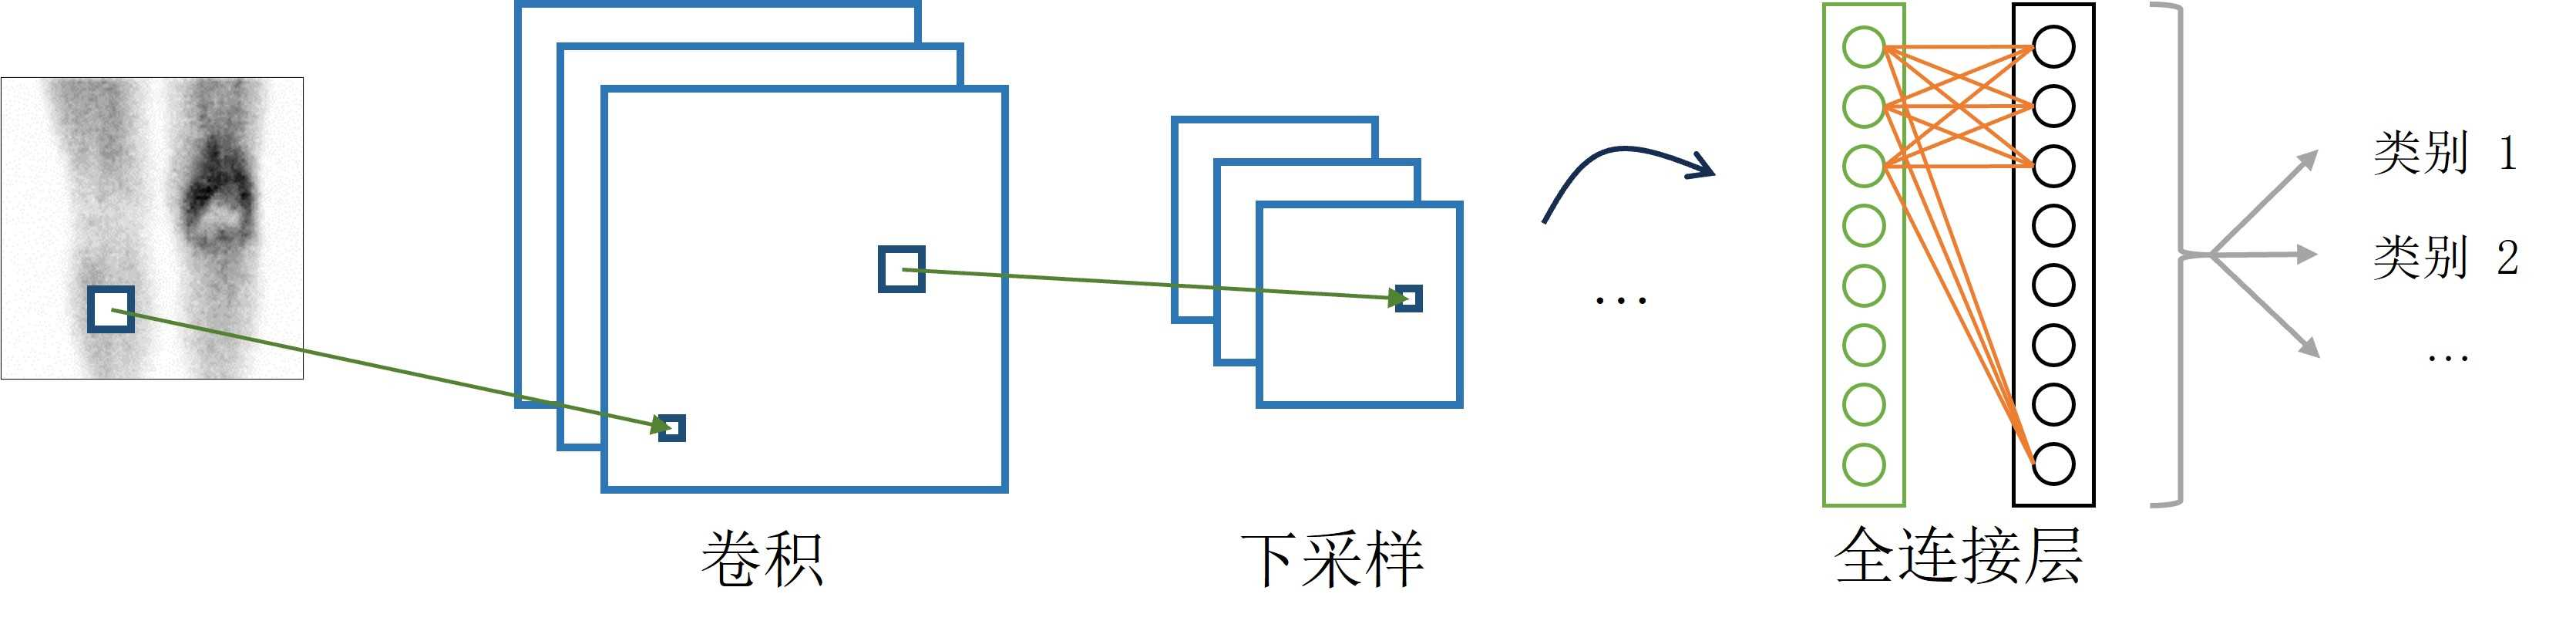
\includegraphics[width=\textwidth]{figures/chap02_cnn.jpg}
  \caption{卷积神经网络示意图}
  \label{fig:chap02_cnn}
\end{figure}

如今,深度学习方法逐渐成为主流,逐步取代了传统机器学习方法的地位。CNN是深度学习方法中具有代表性的方法之一,通常由卷积层,下采样层,全连接层组成,如图\ref{fig:chap02_cnn}所示。卷积层是核心组成部分,最大的特点在于参数共享机制,即通过相同的参数提取输入数据中不同位置的同一特征。参数共享机制可以大大减少参数的数量,提高模型的泛化能力。卷积层中若干个卷积核都具有可学习的参数,而该参数通过梯度反向传播算法进行训练调整。对于输入到卷积层的二维矩阵数据\(I\)而言,输出的像素点\(O_{i,j}\)可由公式\ref{eq:chap02_convolution}表示:
\begin{equation}
  O_{i,j} = \sum_{m=0}^{M-1}\sum_{n=0}^{N-1}I_{i+m, j+n}\times K_{m,n}
  \label{eq:chap02_convolution}
\end{equation}
其中,\(i,\ j\)表示输出矩阵的位置,\(M,N\)是二维卷积的尺寸大小,\(K_{m,n}\)表示卷积核中的权重值。其中,输出图像\(O\)每个位置的值,由卷积核\(K\)会沿着二维矩阵数据\(I\)进行窗口滑动依次计算得出。

接下来将介绍与分析一些经典的CNN模型:LeNet\cite{lecun1998gradient}(1998)是历史上第一个成功应用于手写数字识别任务的CNN,并且为后来的更深层次的CNN的发展奠定了基础。LeNet的整体结构非常简单,一共有七层,包括交替的卷积和池化层,以及全连接层和输出层。它的成功证明了CNN在图像识别任务上的有效性,也使得它成为深度学习领域中里程碑式的模型之一。

AlexNet\cite{krizhevsky2012imagenet}(2012)可以视为第一个现代深度CNN模型,与LeNet有着相似的网络结构,但网络层数更深。它的主要贡献在于:(1)引入了ReLU激活函数去加速训练过程并减轻了梯度消失问题。(2)为了减少过拟合,引入了Dropout\cite{srivastava2014dropout}正则化技术和数据增强方法用以提升模型的泛化能力和鲁棒性并扩充了数据集的大小。AlexNet的出现为后续的CNN的设计和训练提供了重要的启发和借鉴。

VGG\cite{Simonyan2014VeryDC}(2014)的网络结构简单而有效。与AlexNet相比较,它的卷积核更小,都是\(3\times3\)的大小。这不仅可以减少模型参数量,还增加了模型的非线性能力。此外,VGG的网络结构可以更深,通常为16或19层,这使得网络可以捕获更好的复杂特征。VGG在图像分类任务上取得了很大的成功,其清晰的网络结构和易于理解的设计使得它成为了深度学习入门的经典模型之一。

\begin{figure}[ht]
  \centering
  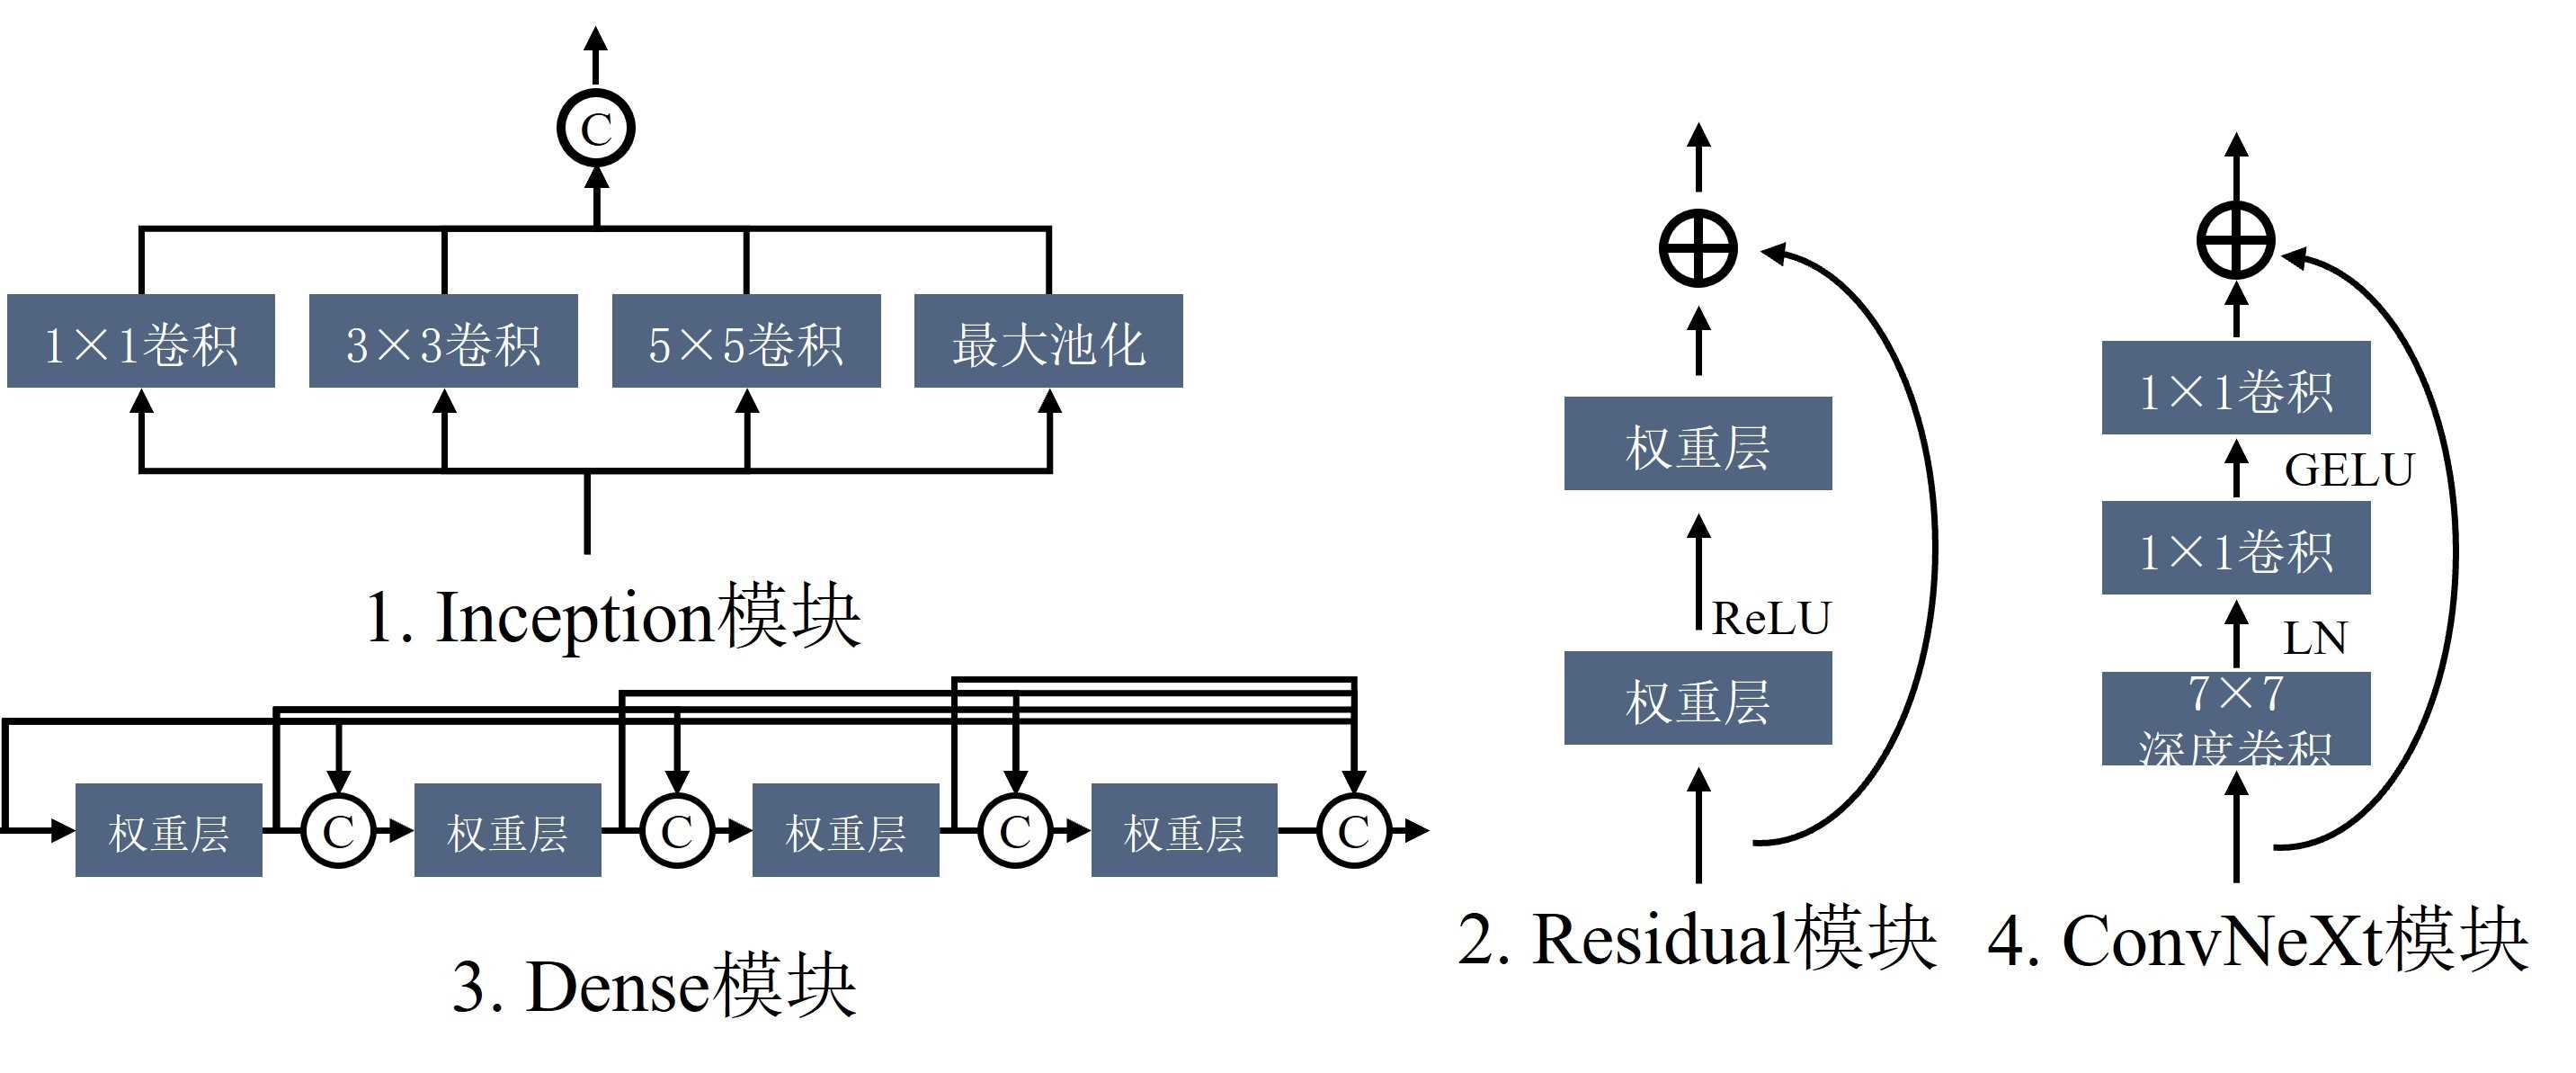
\includegraphics[width=\textwidth]{figures/chap02_block.jpg}
  \caption{不同卷积神经网络的模块示意图}
  \label{fig:chap02_block}
\end{figure}

GoogleNet\cite{szegedy2015going}(2014),也称为Inception网络,初次引入了基础模块(Inception模块,图\ref{fig:chap02_block})的概念,用以搭建一个稀疏且高性能的神经网络模型。Inception模块采用高度并行的设计方式,在多个不同尺度上同时执行卷积和池化操作,以捕获不同层次的特征。它将不同大小的卷积核和池化核组合在一起,让神经网络模型自主学习最合适的特征提取方式。尽管GoogleNet的网络结构为22层,但它的参数量是AlexNet的1/15,同时是VGG的1/3。因此,GoogleNet是在计算资源有限的情况下的一个较好选择。此外,GoogleNet使用全局平均池化层替代了全连接层来整合特征,将每个特征图转换为一个单独的特征值,在大大减少参数量的同时降低了过拟合的风险。

ResNet\cite{he2016deep}(2015)的核心创新点在于引入了Residual模块(图\ref{fig:chap02_block}),用以解决神经网络层数加深时出现的问题,如梯度爆炸、梯度消失以及神经网络模型能力退化。其中,模型能力退化并不是由过拟合造成的,而是由于模型层数的增加导致训练误差的增加。从LeNet到GoogleNet模型发展的历程来看,神经网络模型的网络结构越深,意味着可以提取到越丰富的特征,并且,在更深的网络结构下提取的特征图含有更充足的语义信息。但是实验表明随着神经网络模型不断加深,模型的性能越差。Residual模块通过引入跳跃连接的方式,即将浅层的输入直接与深层的输出相加,保持梯度的流动,提升信息的传播效率,来解决梯度和训练困难的问题。ResNet可以构建非常深的网络,甚至可以超越1000层。相比于传统的网络模型,ResNet更容易优化和训练。ResNet也是深度学习领域中里程碑式的成果之一。

DenseNet\cite{huang2017densely}(2017)在ResNet的基础上更进一步,充分利用了跳跃连接,提出了具有密集连接的Dense模块,如图\ref{fig:chap02_block}。Dense模块为了确保信息的最大流动,将所有层相互连接,其中每个卷积层的输入是前面所有层的特征图拼接而成,输出会保留下来并传给后面所有的层进行拼接。这种密集连接的设计使得网络可以更充分地利用前面提取的特征信息,提升网络模型的表达能力,也有助于解决梯度消失和信息稀疏的问题。DenseNet通过密集连接的设计,实现了全局特征的重用,从而提高了网络对复杂特征的捕获能力。其创新的网络结构和有效的特征融合方式丰富了深度学习模型的设计空间,提供了新的研究思路与方法。

ConvNeXt\cite{liu2022convnet}(2022)从ResNet模型出发,在Swin Transformer\cite{liu2021swin}的设计启发中汲取精华,在网络结构和训练策略上进行了多项改进,得到了性能超越Swin Transformer的CNN。ConvNeXt的基础模块如图\ref{fig:chap02_block}所示。由于Swin Transformer采用较大的自注意力窗口,自注意力中中间隐藏层的特征图通道数更大并且深度可分离卷积与注意力机制的计算具有相似性,ConvNeXt模块采用了倒置瓶颈结构,即中间大、两头小,并使用了大卷积核(\(7\times7\))的深度可分离卷积。此外,在细节优化上,将激活函数ReLu改为了GELU,归一化函数Batch Normalization\cite{ioffe2015batch}改成了Layer Normalization。ConvNeXt表明了纯粹的CNN经过精心设计,依然可以与以Transformer为代表的新兴模型展开竞争。

\begin{figure}[htbp]
  \centering
  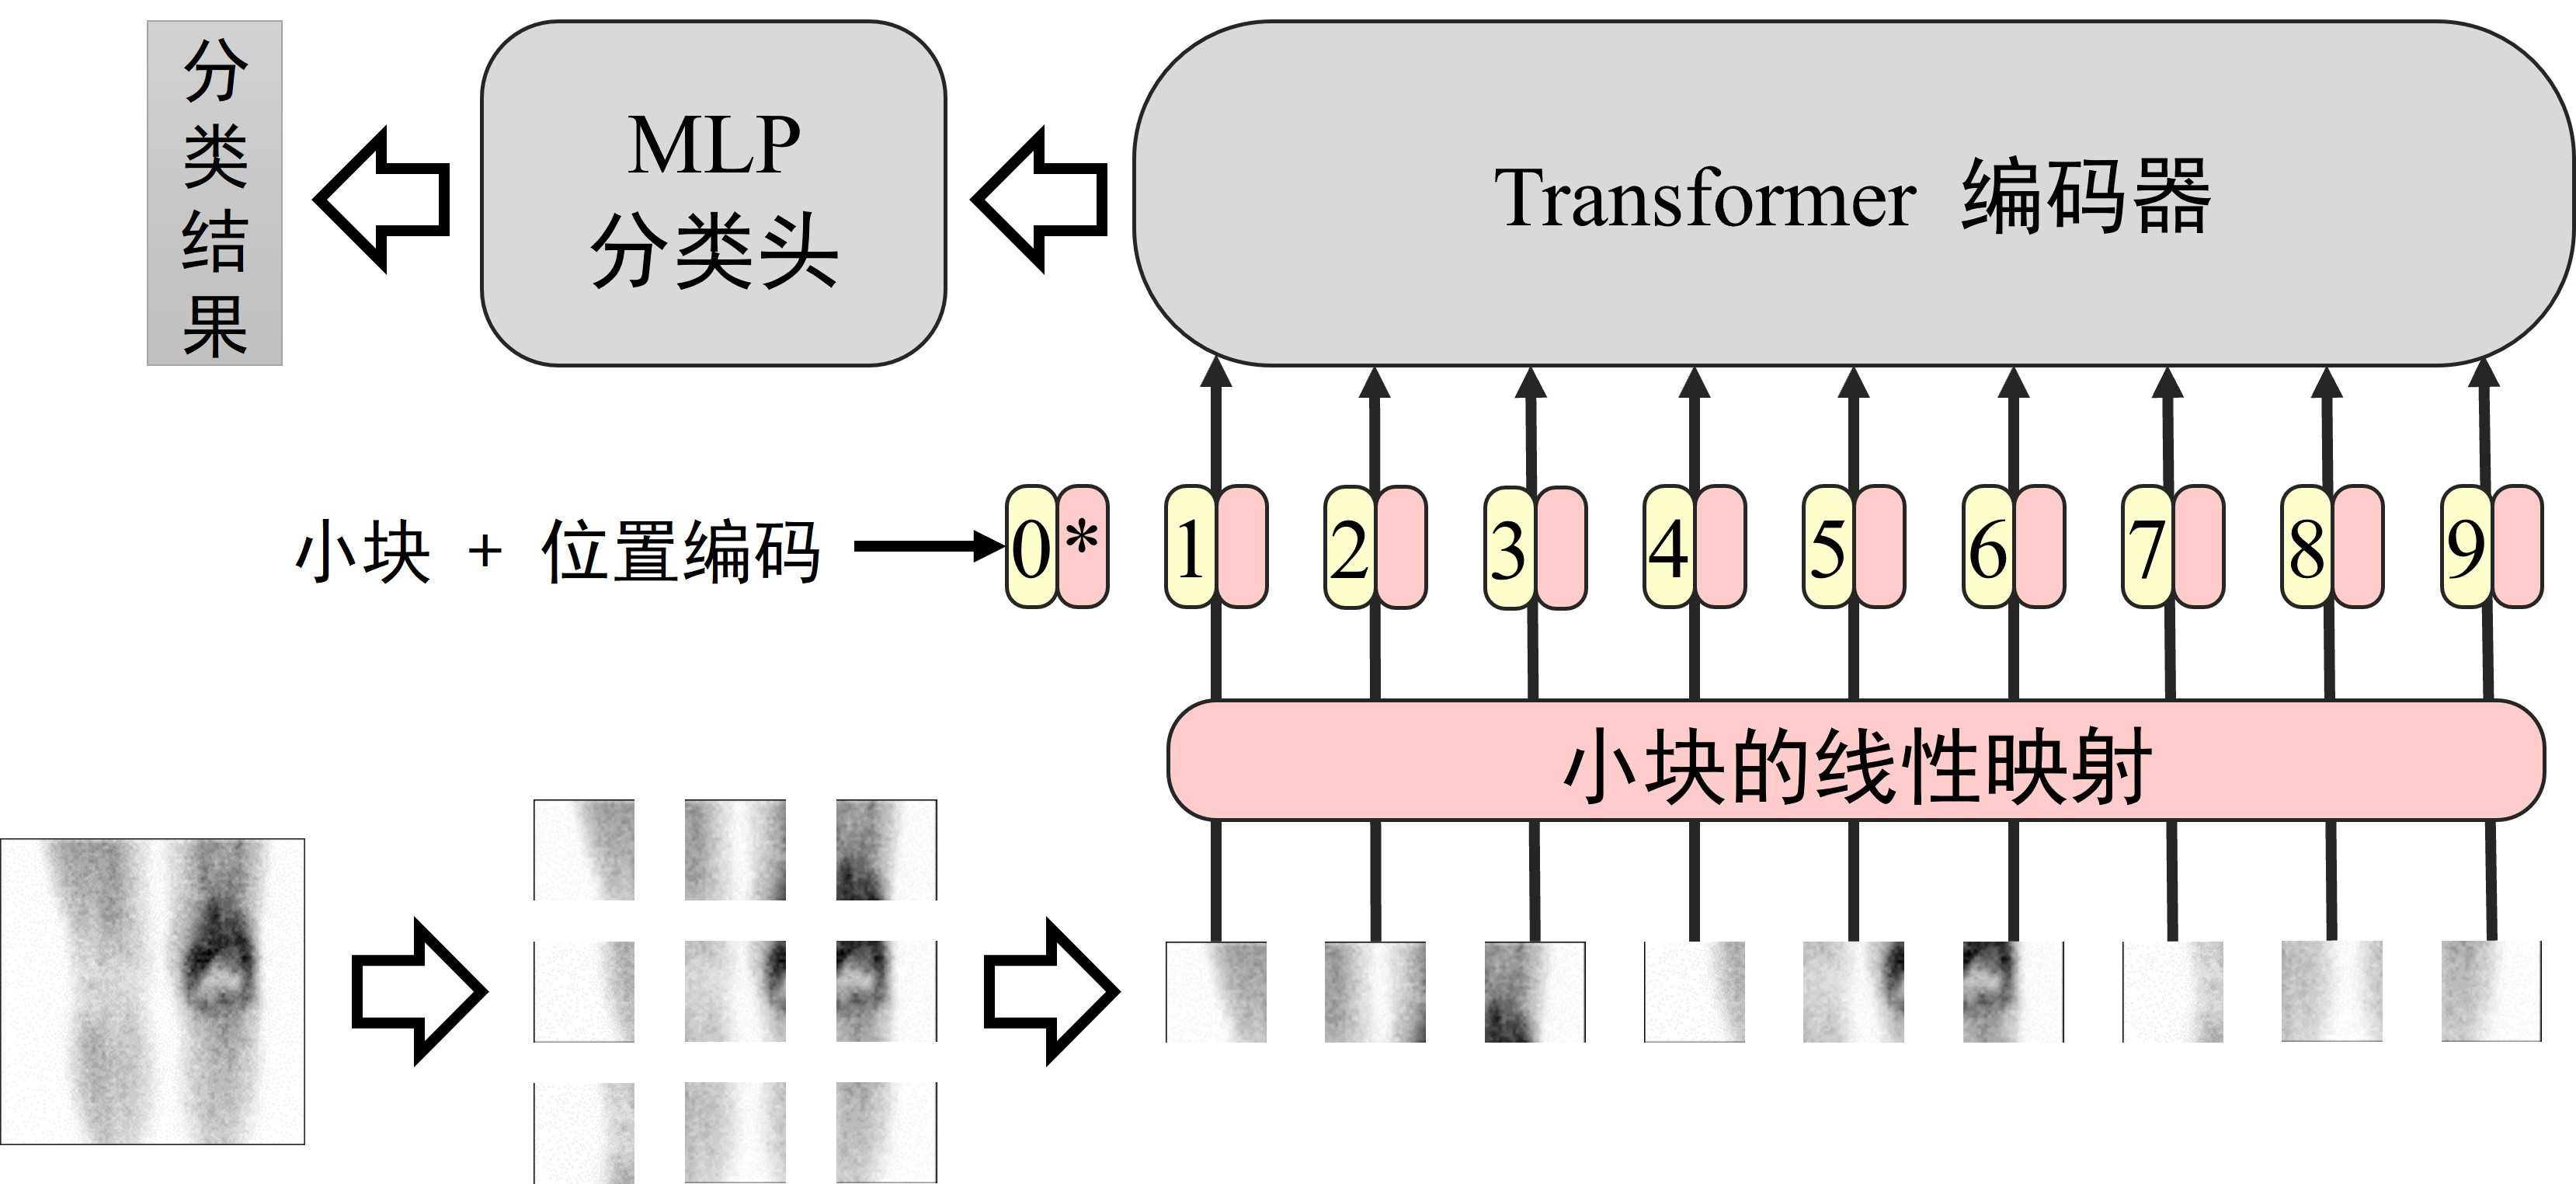
\includegraphics[width=\textwidth]{figures/chap02_vit.jpg}
  \caption{Vision Transformer}
  \label{fig:chap02_vit}
\end{figure}

相比较于CNN,最初为自然语言处理任务设计的Transformer具有一些独特优势。即其自注意力机制在应用于图像时能够全面覆盖整个图像区域并聚焦于高度相关的特定区域。Dosovitskiy等人\cite{dosovitskiy2020image}于2020年的开创性研究引入了Vision Transformer(ViT),这是将Transformer模型成功应用于图像领域的首例,如图\ref{fig:chap02_vit}所示。ViT通过将图片分割成若干固定大小的小块(patches),并为每个小块赋予位置编码后构成序列输入到Transformer网络中。该模型通过捕捉图像中全局和局部的信息,来实现对图像特征的学习与分类。

Swin Transformer\cite{liu2021swin}(2021)是一种新型的Transformer,专为视觉任务设计。其创新之处在于引入了一个称为"shifted window"的机制,它允许跨越多尺度的特征交互。与传统Transformer相比,Swin Transformer通过此机制显著地减少了计算复杂性,使得在处理图像等高分辨率数据时更为高效。其工作原理是将图像分成多个小块,然后在这些小块中局部地应用自注意力机制,之后通过滑动(shift)这些小块的方式实现了全局信息的整合。

Transformer iN Transformer\cite{han2021transformer}(TNT,2021)是另一种创新Transformer架构,它在传统的自注意力机制中嵌入了一个自注意力机制。这个设计的关键是它内部具有两级Transformer结构:第一级抓取像素级的特征,而第二级聚焦于区域特征,从而对整个图像进行特征表示。这种内外Transformer的组合使得这个架构能够更有效地捕获图像内部的复杂结构。

综上所述,CNN和新兴的Transformer都是计算机视觉领域中的强大工具,它们在特征提取和模式识别方面展现出杰出的优势。对于CNN而言,其卷积层具有固定且较小的感受野,这使其能够有效地识别局部特征,如边缘、形状和纹理等,但可以通过多层堆叠以捕捉全局上下文信息。而Transformer通过自注意力机制可以捕捉到全局上下文信息,从而实现对整张图像的理解。然而,Transformer模型的训练需要依赖大量数据,而数据集小是医学影像领域普遍面临的问题。因此,CNN成为了更值得探索的方法。\textbf{对于动态骨显像和PET/CT诊断分类任务而言,CNN可以有效地学习到病灶区域中局部关键性特征,例如生理摄取的形态和解剖结构的细节。然而,对于具有时序性特点的动态骨显像,由于CNN并非专门为处理序列数据而设计,其在这方面的能力是受限的。}

\begin{figure}[htbp]
  \centering
  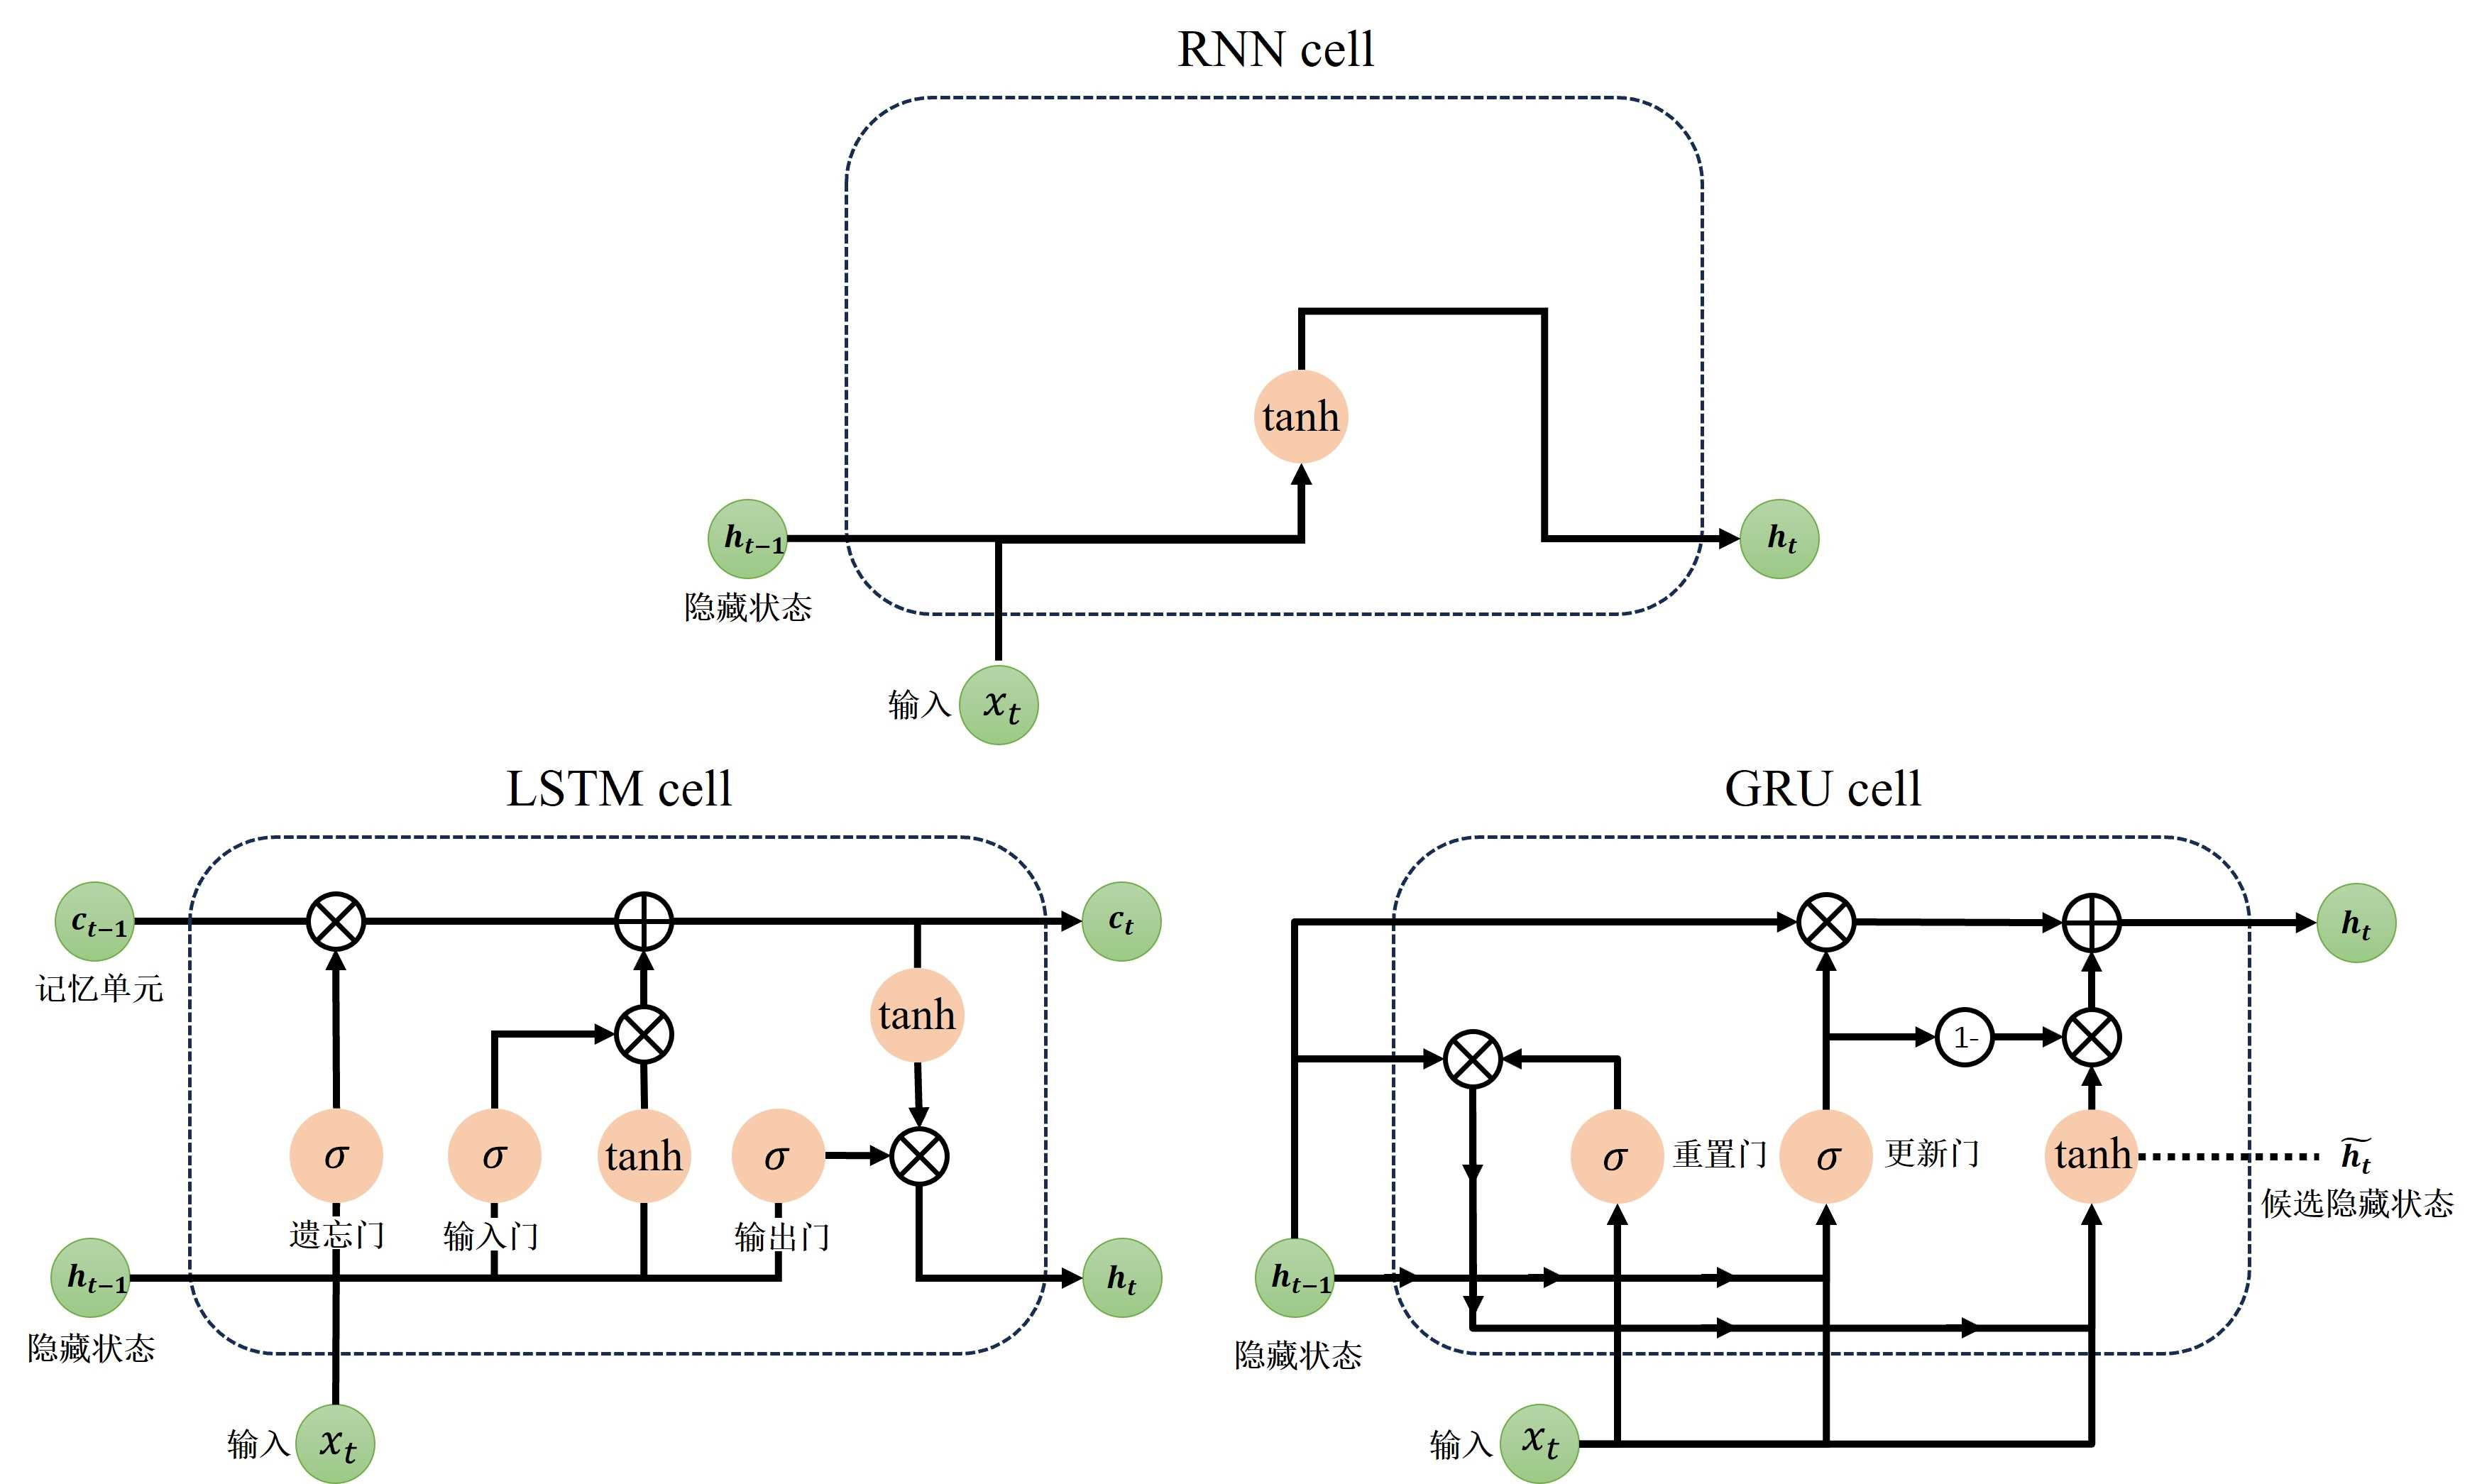
\includegraphics[width=\textwidth]{figures/chap02_rnn.jpg}
  \caption{循环神经网络示意图}
  \label{fig:chap02_rnn}
\end{figure}

对比CNN,RNN作为深度学习方法之一,是一种专门用于处理序列数据的神经网络模型,非常适用于时间序列分析任务之中。RNN的主要原理在于它通过不断地更新隐藏状态(hidden state)去保存序列中每个时间点上一定的历史信息,并用于当前时间点的决策或下一时间点的预测,如图\ref{fig:chap02_rnn}。RNN的结构可以是序列到序列的形式,但当RNN应用于时间序列分析中的分类任务时,其结构可以变成序列到单一输出的形式。对于输入的序列数据\(X = \{x_1, \cdots, x_t, \cdots, x_T\}\)而言,在每个时间点\(t\)上,RNN通过以下公式更新隐藏状态\(h\):
\begin{equation}
  \begin{aligned}
    h_t & = \text{tanh}(W_{h}h_{t-1}+ W_{i}x_t) \\
    y^t & = \sigma_s(W_{h}h_{t-1})              \\
  \end{aligned}
\end{equation}
其中,tanh表示双曲正切函数,\(W_h\)和\(W_i\)分别表示上一隐藏状态到当前隐藏状态的权重和当前输入到当前隐藏状态的权重,\(\sigma_s\)表示Softmax函数,用于计算所属不同类别的概率分布,\(y^T\)表示RNN中的单一输出。

RNN在理论上可以捕捉长期依赖。但是在实际中,随着时间的增长,梯度消失或梯度爆炸的问题会出现,并且RNN学习和保留过去的历史信息的能力是有限的。为了解决RNN中存在的缺陷,研究人员提出了它的变体,长短时记忆网络(Long Short Term Memory, LSTM)\cite{memory2010long}和门控循环单元(Gated Recurrent Unit, GRU)\cite{chung2014empirical}。

LSTM\cite{memory2010long}(2010)相比较于RNN拥有一个更为复杂的结构,如图\ref{fig:chap02_rnn}所示。它在RNN的基础上添加了三个门控记忆单元(遗忘门、输入门和输出门)以及一个独立的记忆单元\(c_t\)来更新和输出隐藏状态。在长序列数据的处理中,LSTM展现出其强大的能力,通过动态地调节记忆单元,以实现时序信息的有效保留。在训练过程中,LSTM通过精确的门控机制,执行三项关键操作:首先,它利用遗忘门从单元状态中丢弃非核心信息;其次,它通过输入门引导新的信息加入单元状态;最终,它通过输出门精心挑选必要信息来构建输出。这一过程赋予了其在长时间跨度上维持和更新历史信息的能力,并捕捉到数据的深层依赖关系。由此机制,LSTM有效地克服了传统RNN面临的梯度消失与梯度爆炸问题。

GRU\cite{chung2014empirical}(2014)相比较于LSTM,简化内部繁琐的门控机制,如图\ref{fig:chap02_rnn}所示。它在LSTM的基础上将隐含状态与记忆单元合并为一个统一的隐藏状态,并通过两种门控单元(更新门与重置门)来控制信息流动。更新门的作用是调节前序隐藏状态对当前隐藏状态的影响程度,允许模型在必要时保存跨越较长时间区间的信息。而重置门则决定在当前隐藏状态的更新过程中,前序隐藏状态的参与程度,这样使得模型可以有选择性地忘记或保留过往信息。GRU通过更加灵活和精简的门控策略来维持长期的状态信息,并同时捕获短期的上下文特征,这一策略在许多实验中被验证能够有效预防梯度消失的问题。

Yiugit等人\cite{yiugit2021simple}于2021年提出了两种简单且有效的GRU变体:GRU1和GRU2。通过一种基于经验的方法,这些学者试图确定一组能够提高GRU准确度或降低损失的系数\(\epsilon,\alpha\)。其中,\(\epsilon\)确定门控循环单元的作用力度,\(\alpha\)确定门控当前单元门的作用力度。相比较于GRU,GRU1增加了当前单元的作用,而GRU2减少了循环单元的作用。值得说明的是,对标准GRU算法进行这样微小且简便的调整能够显著提升其性能。

综上所述,RNN及其变体为处理序列数据提供了富有弹性的学习架构。RNN以其简单的循环连接结构,去捕获时序信息,但仍存在梯度消失或爆炸的问题。LSTM和GRU则引入门控机制,有效地保存长期依赖关系,优化了信息的存储与过滤,降低了梯度消失和爆炸的风险。\textbf{对于动态骨显像中的假体关节感染诊断任务而言,不仅需要关注每张图像中的病灶摄取形态特征,还需要抓取跟时序相关的生理代谢差异变化特征,RNN和CNN的有效结合将适用于该任务的模型设计,同样也是图像序列分类任务的重点研究方向之一。}

\subsection{医学影像分类算法}

计算机辅助诊断(computer aided diagnosis, CAD)是通过计算机对病患的医学影像,如PET、CT、MRI等,进行分析并辅助医生完成相应疾病的诊断流程。计算机依靠逐渐流行的深度学习技术,可以自动地从目标数据中学习获得更深层次的特征,并且排除人为因素的影响,实现全自动化的辅助诊断。基于医学影像的分类诊断是计算机辅助诊断的重要研究方向之一。对于不同的医学影像而言,由于其本身的成像技术不同,从而拥有不同的特性和成像效果,这也是科研人员不可忽视的研究基础之一。根据医学影像的特点,有效设计合适的图像处理算法和模型结构有助于提升分类诊断任务的质量。

Cheng等人\cite{cheng2017classification}(2017)提出了一个级联的三维CNN用于脑部PET影像的分类诊断。该方法首先划分整个PET脑影像为数个三维的局部子区域。接着,利用一个三维卷积网络来提取每个子区域中更深层次的鉴别特征。最后,应用一个高级别的三维卷积网络来融合各个子区域特征,实现对阿尔茨海默症患者与健康对照组的有效区分。
Liu等人\cite{liu2018classification}(2018)在阿尔茨海默病的诊断领域,采用了创新性的方法,将CNN与RNN相结合。把三维PET影像分解为二维切片序列,通过二维卷积网络学习切片内部的特征和RNN掌握切片间的序列特征,来展现对阿尔茨海默病的高效分类性能。
Khagi等人\cite{khagi2020cnn}(2020)提出了一种用于脑部MRI和PET影像进行分类诊断的三维卷积架构divNet。它可以有效区分阿尔茨海默症、轻度认知障碍和正常,用于协助临床医生进行初步快速检测来确定患者的病情。
Lee等研究者\cite{lee2021performance}(2021)对PET影像进行了深入探究,评估了Inception3D、ResNet3D以及VGG3D三种深度学习架构在阿尔茨海默病诊断中的性能表现。结果显示,这些模型在诊断任务中平均准确率高达95\%。在进一步的外部验证中,VGG3D具有最佳的泛化能力。
Liu等人\cite{liu2022diagnosis}(2022)提出一种创新性多尺度CNN来用于脑部MRI影像中的阿尔茨海默病的诊断。该网络通过引入通道注意机制,改善通道间的相互依赖关系,自适应地调整通道维度上的特征,来增强它的特征表达能力。大量实验证明,通过将MRI划分为白质(white matter) 和灰质(gray matter)来进行训练,该网络以更少的参数和更低的计算复杂度获得了最优异的性能。
Takahashi等人\cite{takahashi2022deep}(2022)探索了一种创新的图像预处理方式,即采用了多角度的最大强度投影(Maximum Intensity Projection,MIP),如图\ref{fig:chap02_mip}所示。他们将MIP预处理后的三维PET影像输入至深度学习模型中进行训练,使其能够识别乳腺癌的标志性特征。在随后的性能评估中,该模型展现出了超越没有经验的放射科医生的诊断能力,与三名专业放射科医生相当的诊断能力。

\begin{figure}[htbp]
  \centering
  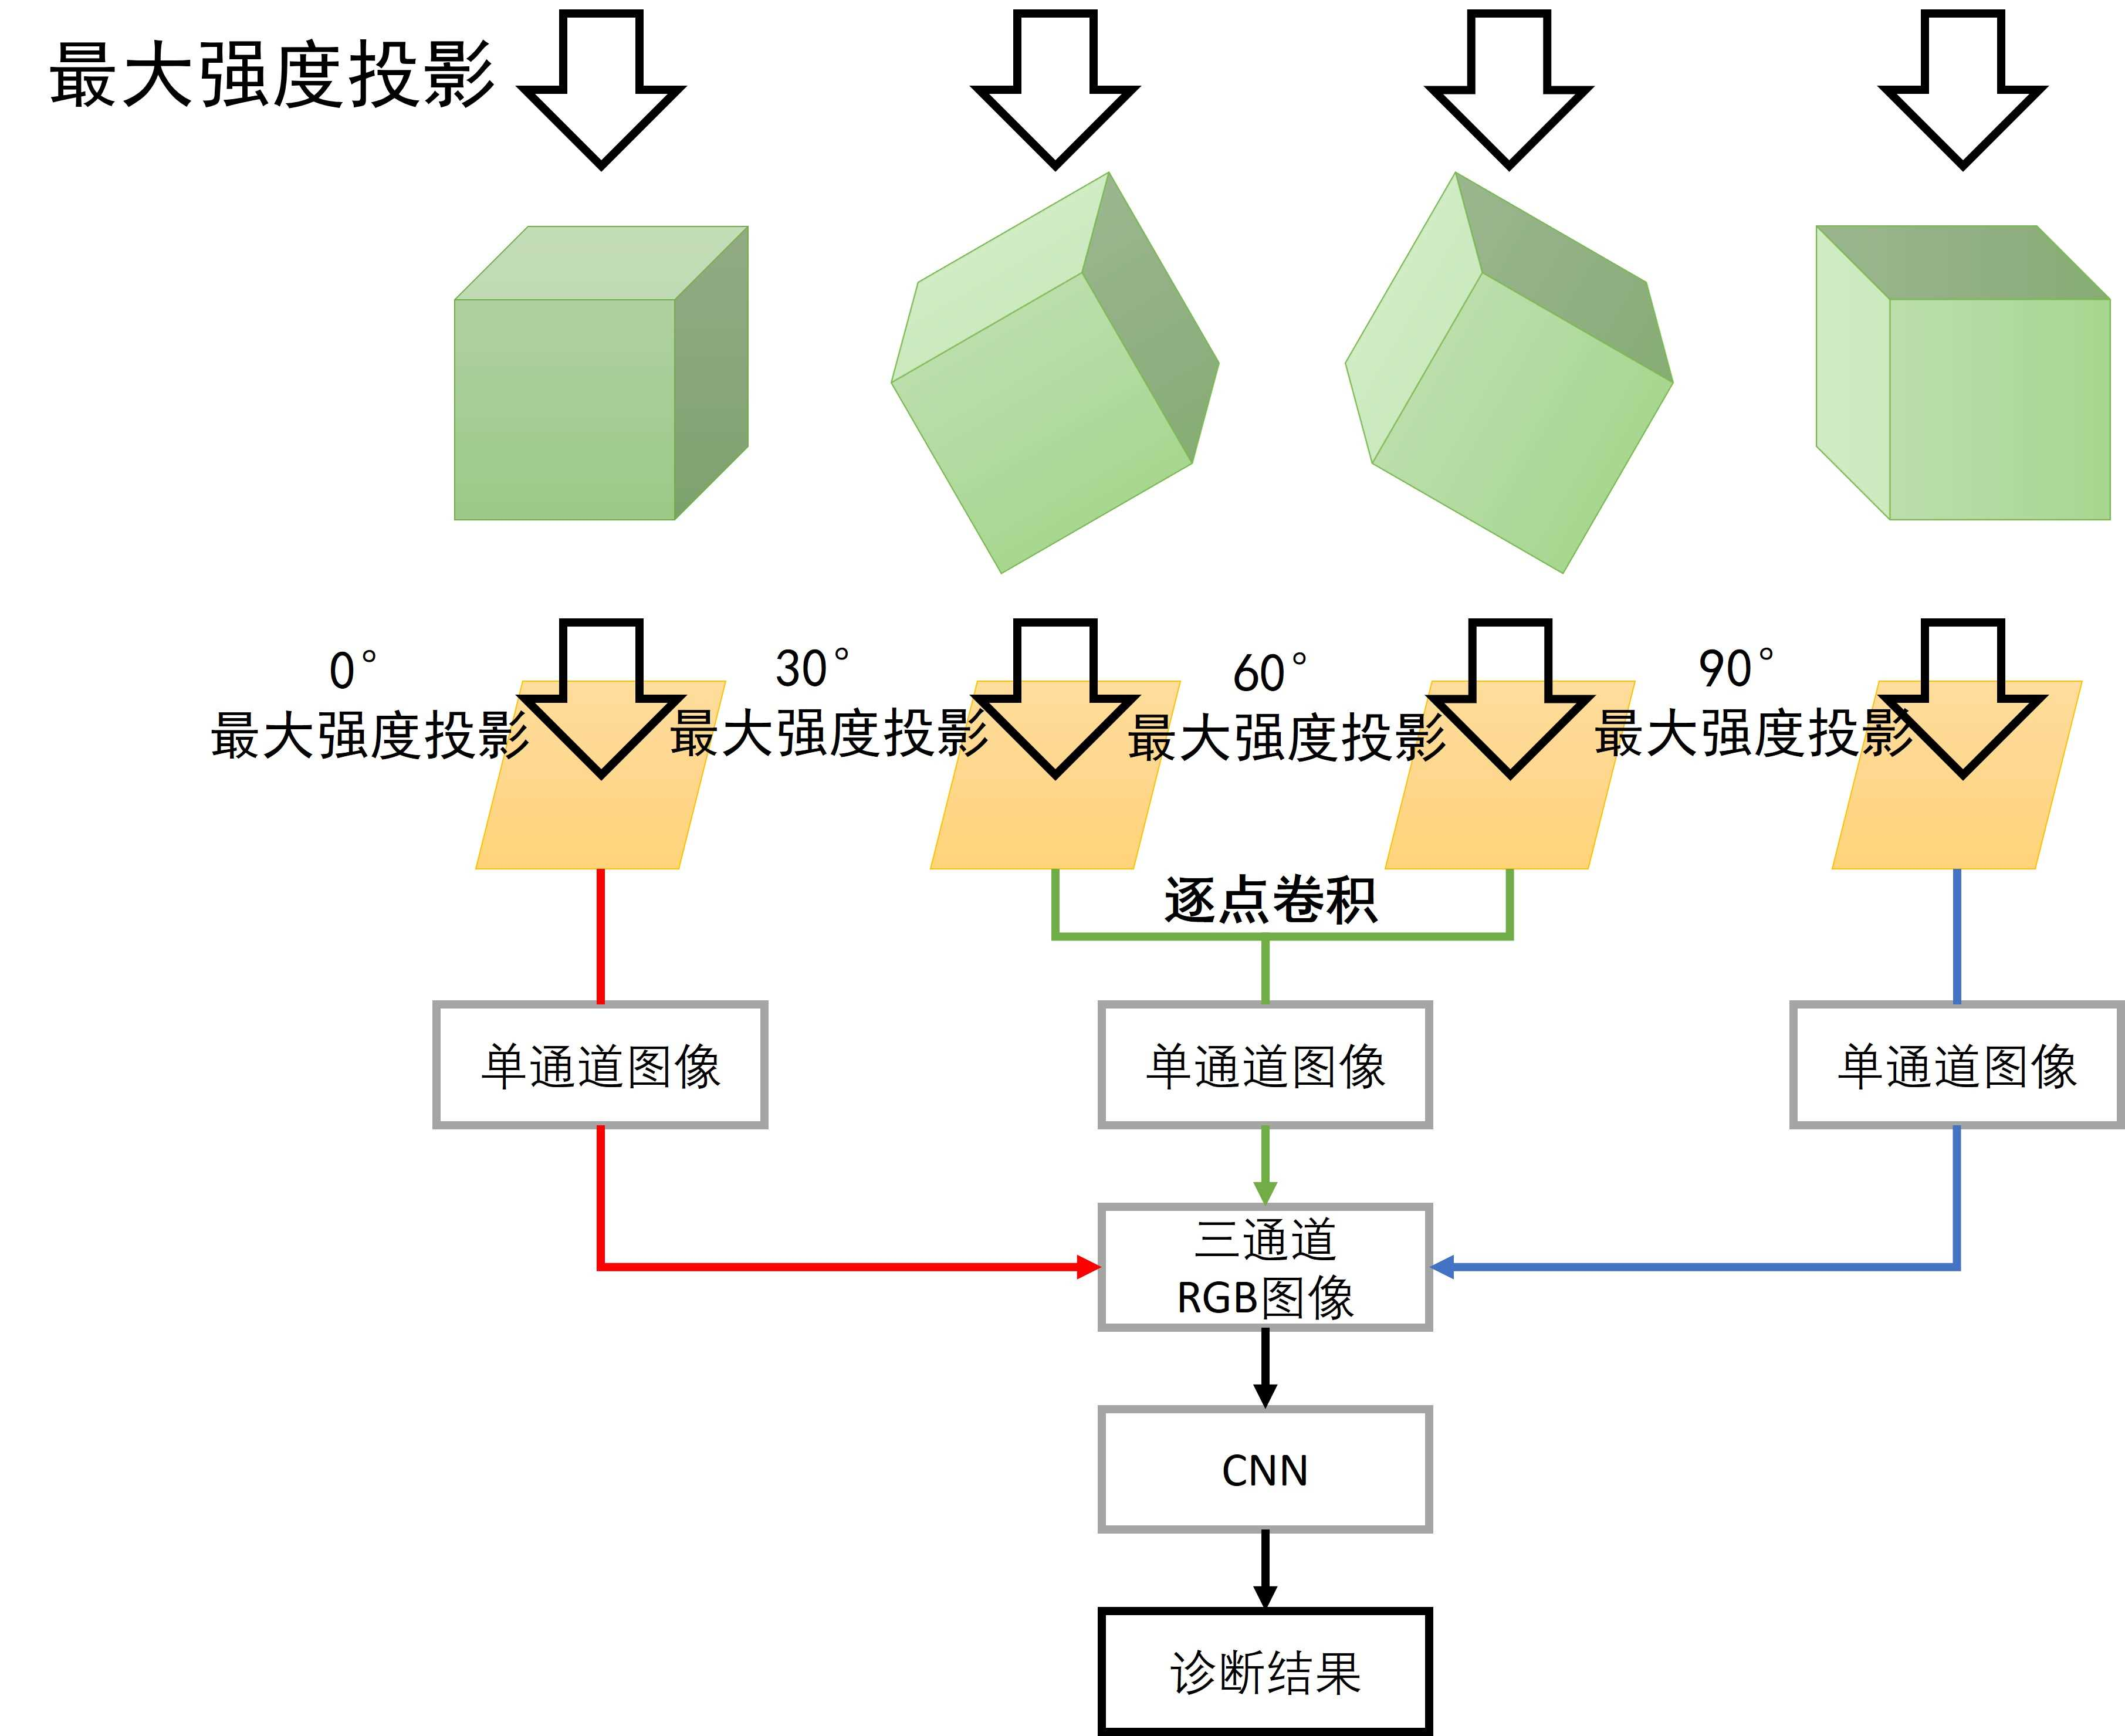
\includegraphics[width=0.8\textwidth]{figures/chap02_mip.jpg}
  \caption{最大强度投影四个角度的图像输入到卷积神经网络进行预测的示意图}
  \label{fig:chap02_mip}
\end{figure}

\textbf{综上所述,对于动态骨显像中假体关节感染任务,以上研究存在一些可借鉴之处。}例如,将时序性图像的固有三维性质,直接采用三维CNN进行特征提取似乎是一种直观的策略。然而,传统的CNN在捕捉长期时序依赖方面存在局限性。\textbf{由此,结合使用CNN和RNN,以便在时间序列的内部和之间提取综合特征,对于该特定医学任务来说可能更加精准和适宜。}同时,也应该重视任务的特定难点,比如无关区域干扰和生理状态下高摄取区域可能对分类精度造成的负面影响。\textbf{鉴于此,研究并设计针对动态骨显像的数据预处理方法,去有效减少负面影响,进一步优化深度学习模型的性能,是提高诊断精准度的关键。}

\textbf{在PET/CT影像中的骨折相关感染任务中,}考虑到PET/CT为三维影像数据,直接采用三维CNN是一个不错的选项,以便充分利用体积数据的空间信息。同时,\textbf{考虑到计算复杂度和数据维度的挑战,采用MIP对数据进行降维处理也是一个有效的替代方案。}此外,针对PET/CT影像的特定情况,如多病灶的存在和相对较小的病灶区域在整体影像中难以突显导致传统的深度学习模型可能无法有效集中于关键的病灶区域的问题,需要特别关注。\textbf{因此,开展针对PET/CT影像的专门预处理方法和引入检测算法定位病灶区域,并对其进行截取或突出处理,可以在不损失重要信息的前提下减少背景噪声的干扰,进而提高深度学习模型在骨折相关感染检测任务中的准确性和效率。}

\section{图像检测}

检测任务通常指输入数据中一个或多个目标物体的识别与空间定位过程。图像检测,在计算机视觉领域内,是解决“识别图像中存在的目标对象以及这些目标对象的准确位置”的关键性问题。该任务适用于众多领域,例如安防监控、自动驾驶、医学影像分析等等。

在医学影像分析中,检测任务特别强调了对疾病标志物的精准定位与识别,如肿瘤、异常组织等,从而为临床诊断提供关键的影像学依据。随着深度学习技术的发展,检测任务通常是要求模型通过边界框来准确发现并定位目标对象。在深度学习与医学影像分析相结合的背景下,检测任务有时会通过像素级分类,即图像分割,来增强目标的定位精度。无论是哪种定位方式,这都需要检测模型具有理解和区分图像中各种复杂特征的能力,以便实现对不同的目标对象的准确识别和区分。

在骨折相关感染的诊断流程中,医生通常集中审视病灶区域在生理代谢方面展现的摄取形态,因为与感染相关的特征通常紧密聚焦于这些区域。对此,探讨检测任务中的神经网络架构显得尤为重要。本节将概述有关于此方面的研究现状,并分析这些架构应用于PET/CT影像上进行骨折相关感染病灶区域检测的可行性。

\subsection{图像检测算法}

在执行检测任务的深度学习模型分类上,一般可划分为目标分割模型与目标检测模型两大类。目标分割模型,以U-Net\cite{ronneberger2015u}为代表,旨在实现对图像中每个像素所属类别的识别,从而获取精确的目标形状与位置。这类模型在医学影像中尤为重要,因为它允许细致划分病灶区域,为后续的量化分析提供了基础。相对地,目标检测模型,如区域卷积神经网络(Region with CNN features,R-CNN)\cite{girshick2014rich}和YOLO(You Only Look Once)\cite{redmon2016you},往往通过预测边界框来定位目标对象,提供了一种相对较快且效率更高的检测方法,尽管其定位的精细程度相对较低。无论是哪种类型的模型,其设计和优化都在不断地促进医学影像分析与计算机视觉领域的研究进展,继而改善临床诊断与治疗的质量。

\begin{figure}[htbp]
  \centering
  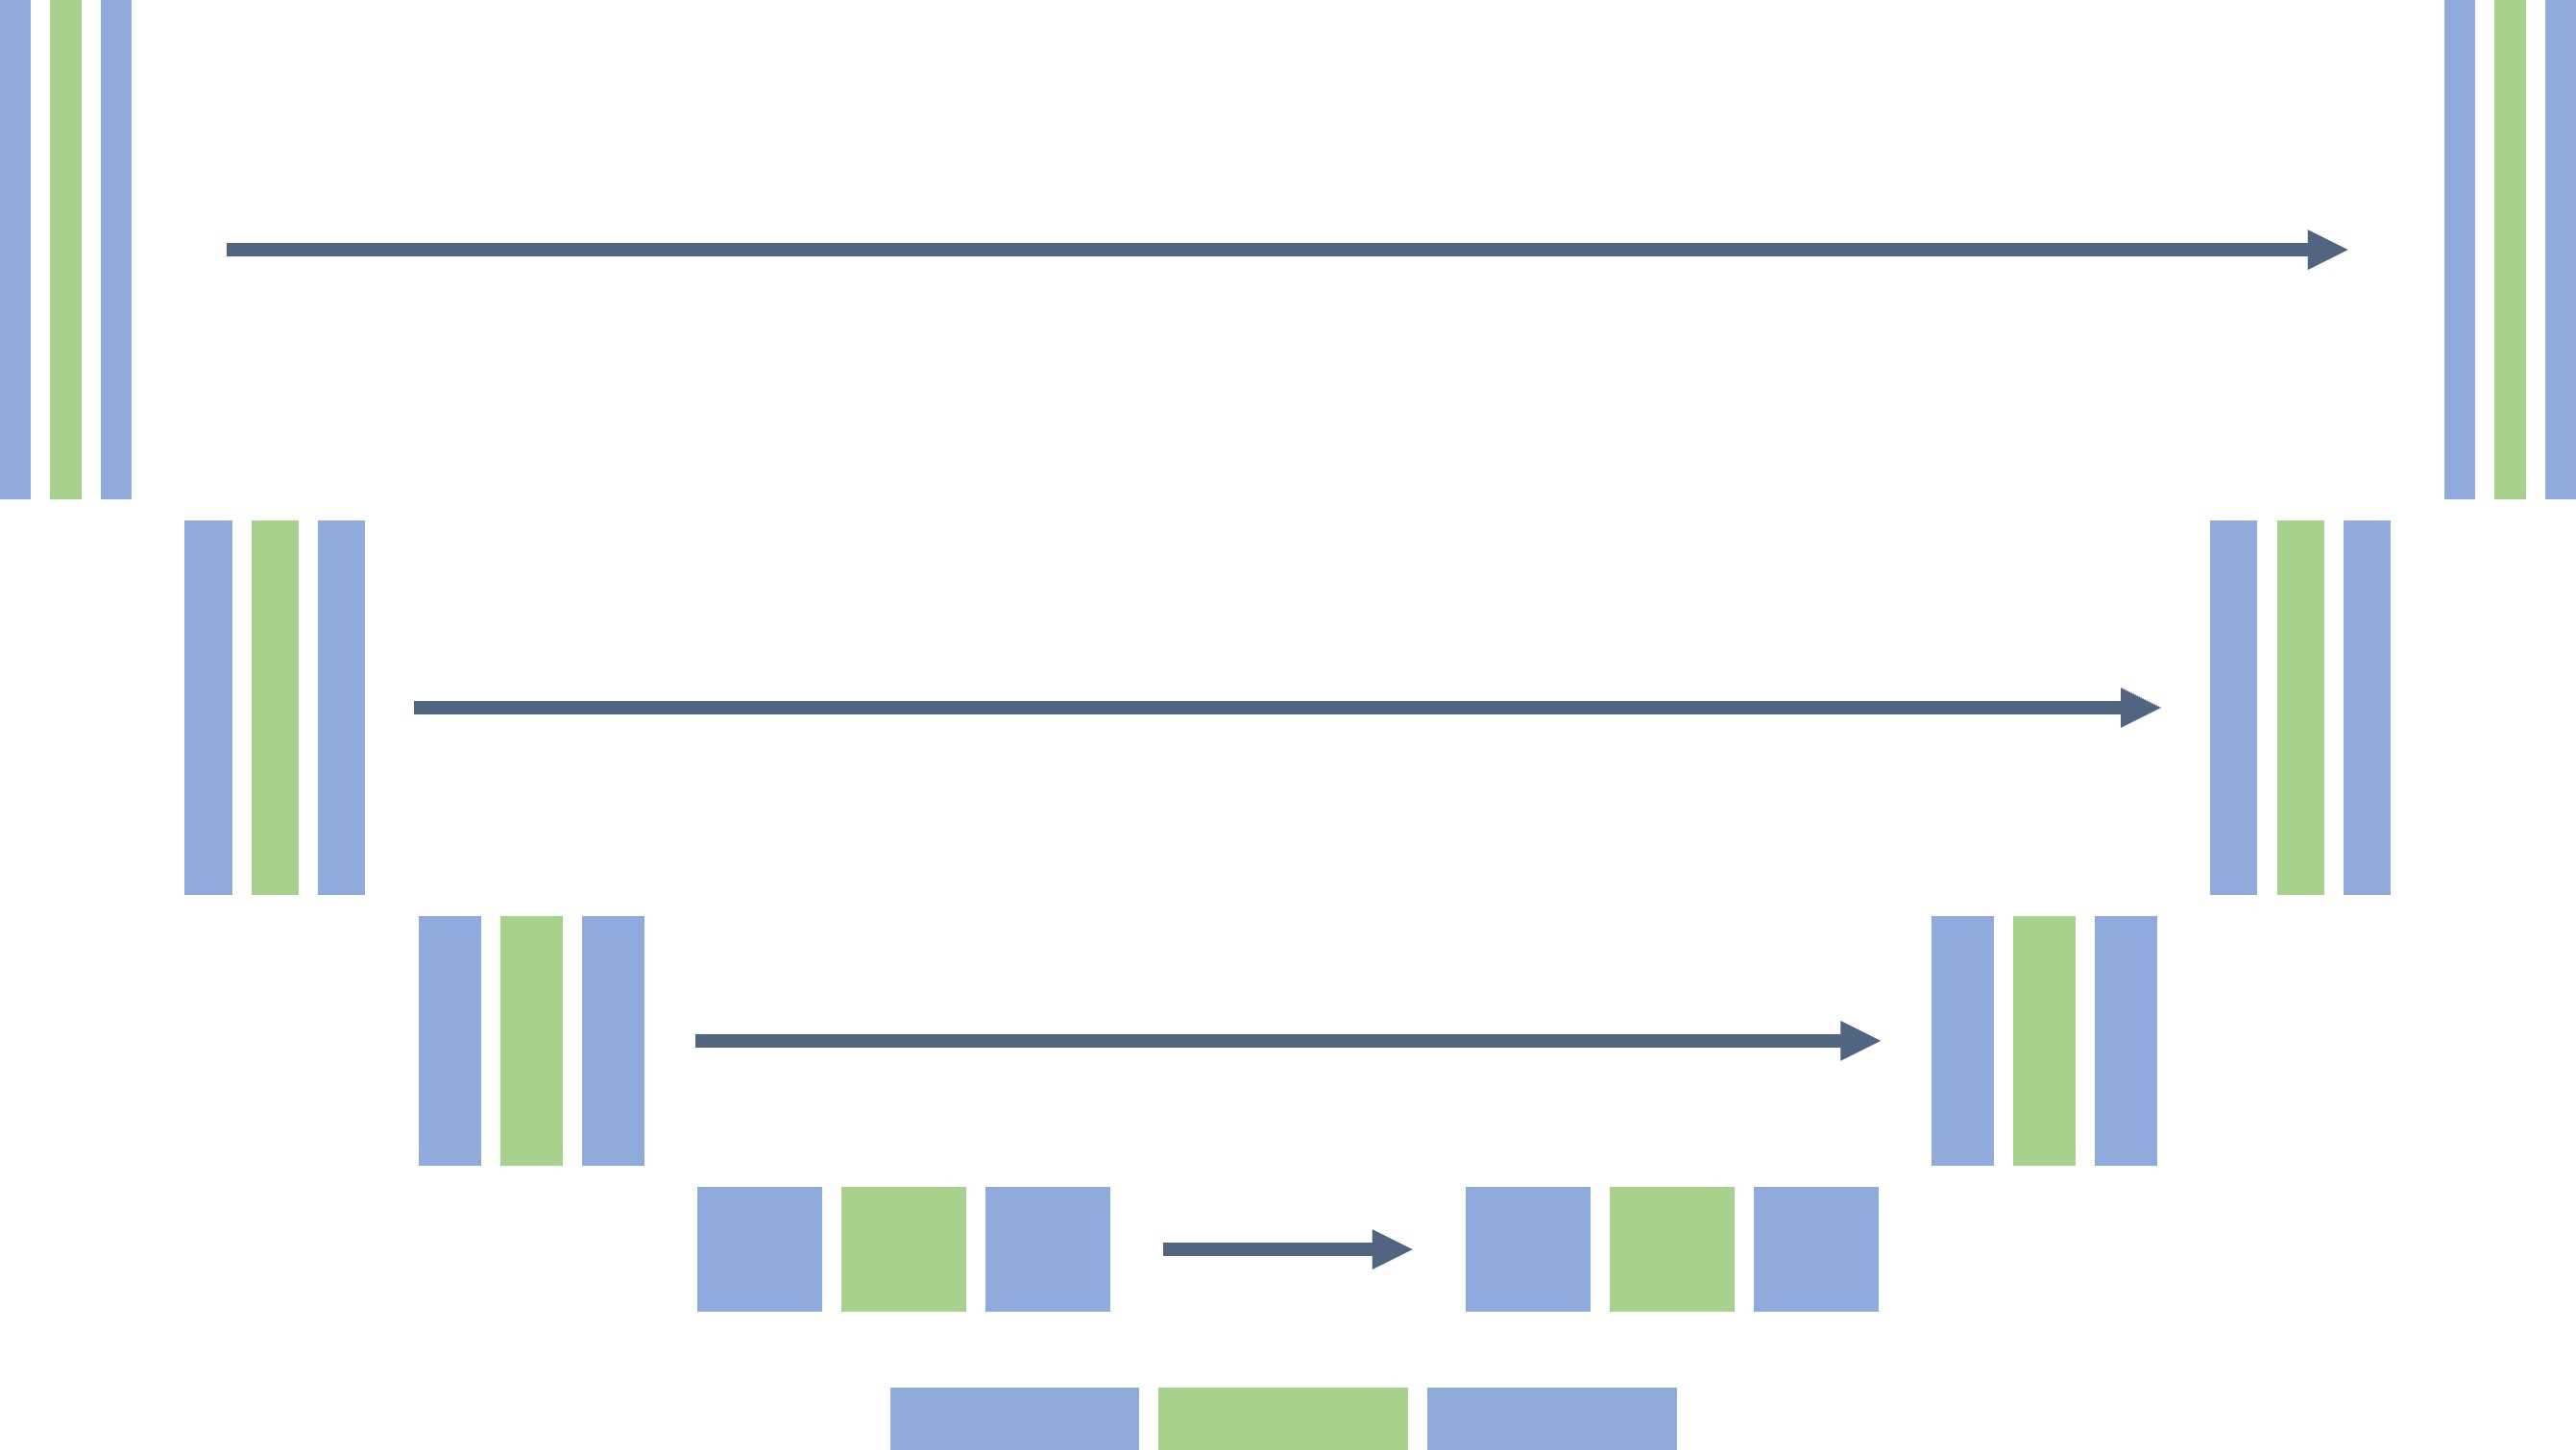
\includegraphics[width=\textwidth]{figures/chap02_unet.jpg}
  \caption{U-Net整体结构示意图}
  \label{fig:chap02_unet}
\end{figure}

在目标分割模型中,U-Net\cite{ronneberger2015u}(2015)的提出开辟了医学影像分割任务的新纪元。它是一种专为医学图像分割设计的深度学习模型结构,摒弃了之前模型对大量数据依赖的限制,在较少标注样本的情况下仍能实现高效能的模型训练。在结构上,如图\ref{fig:chap02_unet}所示,整体呈现为一种“U”字形的对称结构,包括下采样(收缩路径)和上采样(扩展路径)两个部分,能够捕获上下文中多尺度的语义信息。下采样阶段逐步提取特征并降低数据维度大小,而上采样阶段逐步恢复数据维度大小并进行特征解码。同时,通过跳跃连接将下采样阶段的语义信息与上采样阶段的位置信息相结合,以增强特征并实现精确的定位。

U-Net++\cite{zhou2018unet++}(2018)是U-Net\cite{ronneberger2015u}的嵌套版本,强化了特征学习能力,增强了模型对复杂医学影像的分割准确度。主要的创新点包括跳跃连接的重新设计和深度监督。在跳跃连接方面,U-Net++添加了密集的跳跃路径,允许模型结合来自不同阶段的特征,从而提升了捕捉细节、特征融合与学习的能力。在深度监督方面,U-Net++为了充分利用多尺度的语义信息,在每一层的嵌套路径上,都可以输出一个分割图结果。通过所有的分割图结果一起联合优化,有效地强化了模型对不同尺度特征的学习。

Attention U-Net\cite{oktay2018attention}(2018)是一种集成了注意力机制的改进型U-Net\cite{ronneberger2015u}。这种机制可以使得模型更加关注于影像中的关键部分,从而提高特征的区分力和医学影像分割的准确性。其核心的创新点在于跳跃连接中加入了注意力门控模块,以便过滤和引导传统的跳跃连接特征,使得网络能够集中学习更有价值的信息。

U-Net 3+\cite{huang2020unet}(2020)是在U-Net的基础上发展出来的一种医学影像分割模型。该模型通过引入全尺度跳跃连接和深度监督机制,增强了对多尺度特征的融合,并提高了模型的学习能力。全尺度跳跃连接保证了各个解码阶段中全尺度特征的充分利用,而深度监督机制在各个解码阶段直接引入了额外的监督,确保了模型在多层结构上的有效特征学习和提取。

TransU-Net\cite{chen2021transunet}(2021)是一种结合了卷积强大的局部特征提取能力和Transformer的全局自注意力机制的新型网络架构。它先使用卷积提取空间特征,再利用Transformer编码器以捕获长距离上下文关系,最后通过解码器来输出精确的分割结果。这种混合架构使得TransU-Net在分割精度上超越了传统的CNN网络。

综上,U-Net及其变体具有强大的特征学习能力,在医学影像处理中得到了广泛的应用。每个变体都是为了解决特定问题而设计,比如改进特征的捕获能力、更精确地分割图像中的特定部分等。随着深度学习技术的进步,将会有更多的U-Net变体被提出来解决更复杂的医学影像分割任务。\textbf{在PET/CT中,用于识别骨折相关感染病灶的任务面临的挑战在于感染区域的形态分布呈现多样性,包括但不限于点状、簇状或弥散性分布。这种分布的复杂多样性导致利用像素级定位进行精确标注和检测变得较为困难。因此,本研究的重点在于目标检测模型。}

在目标检测模型中,深度学习方法主要分为两大类:二阶段检测器和一阶段检测器。

\begin{figure}[htbp]
  \centering
  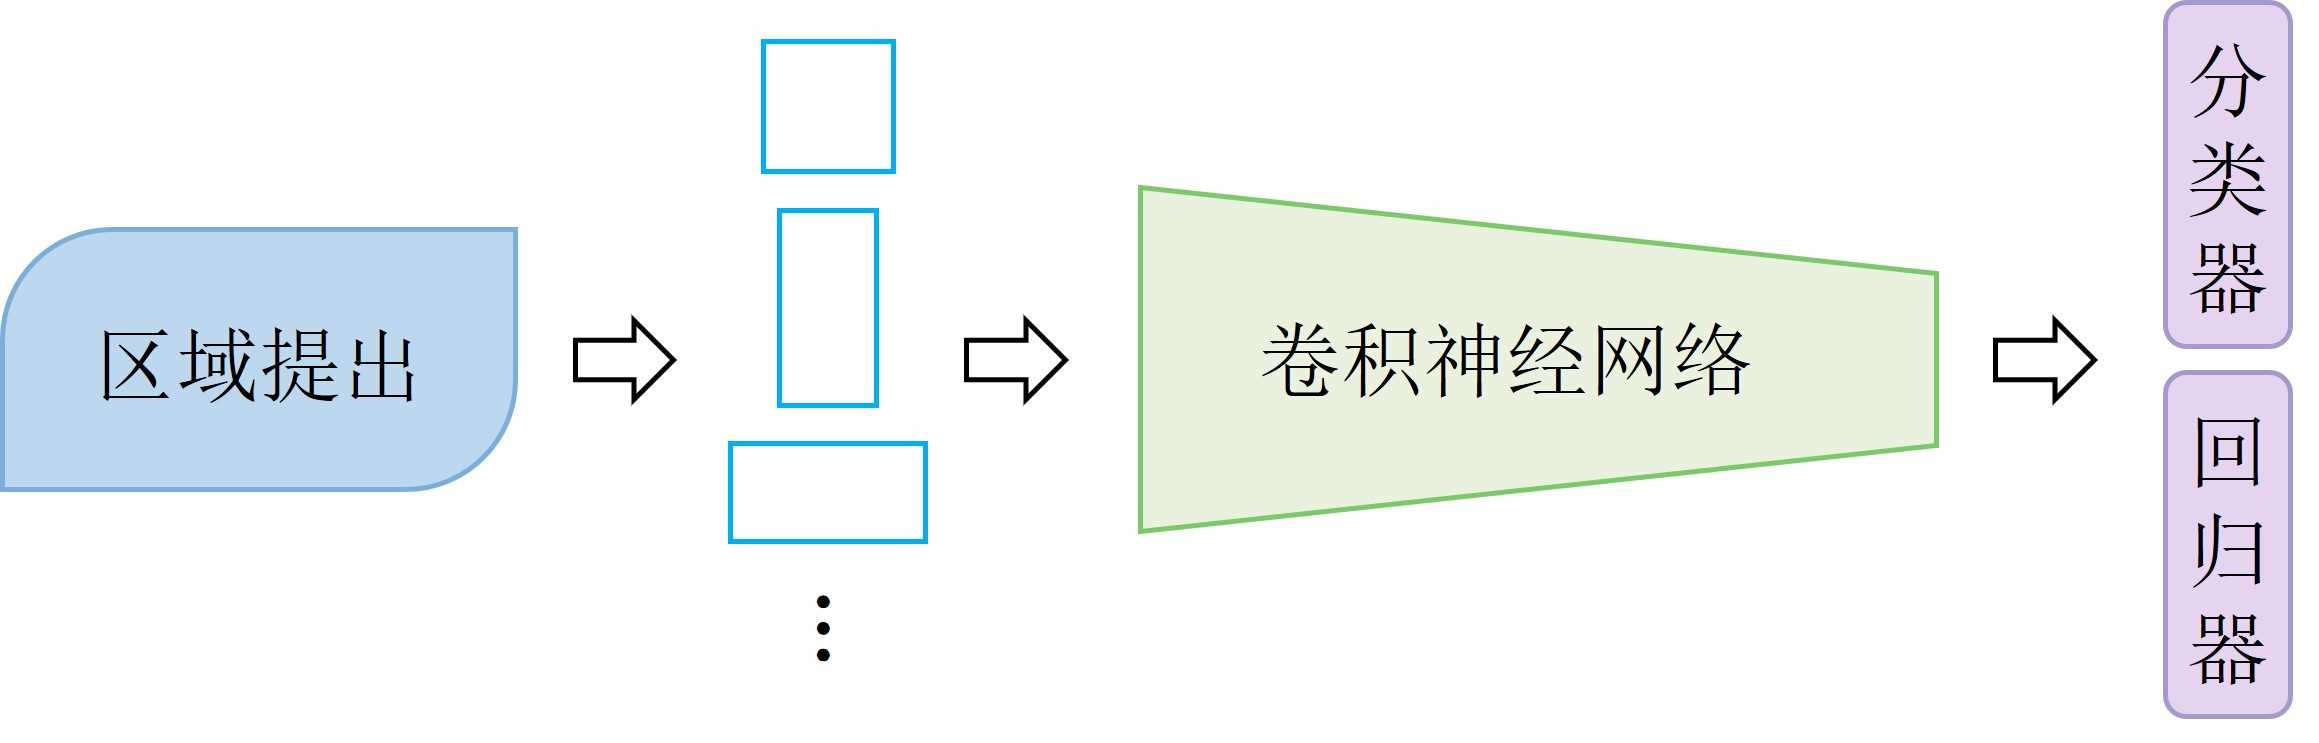
\includegraphics[width=0.8\textwidth]{figures/chap02_rcnn.jpg}
  \caption{R-CNN整体结构示意图}
  \label{fig:chap02_rcnn}
\end{figure}

二阶段检测器的工作流程分为两个阶段:1.生成目标的候选区域;2. 提取这些区域的特征进行分类和边界框的精调。在具有里程碑式的二阶段检测器中,R-CNN\cite{girshick2014rich}(2014)是第一个开创性的二阶段检测器,整体结构如图\ref{fig:chap02_rcnn}所示。在R-CNN模型中,首先由选择性搜索(Selective Search)算法依据图像特征如颜色、纹理、形状等,负责挑选出潜在含有目标对象的候选区域。随后,对这些区域进行标准化预处理,并通过预训练的CNN提取特征。最终,由分类器对特征区域进行分类,并通过边界框回归器精确调整目标对象的位置,以提升目标检测的准确性。虽然R-CNN在其推出时对目标检测领域产生了巨大的影响,但它也存在一些缺点,例如速度慢、训练需要对不同部分分阶段进行,存储需求高。为了克服这些缺陷,后续基于R-CNN的改进模型,如Fast R-CNN\cite{girshick2015fast}和Faster R-CNN\cite{ren2015faster},被提出。

Fast R-CNN\cite{girshick2015fast}(2015)对整个目标检测流程进行了端到端的优化,使得模型可以同时执行目标分类任务和目标定位任务,从而提高了训练速度、检测效率和检测精度。该方法的核心创新点有两个:一是共享了CNN提取的整个图像的特征,采用了感兴趣区域池化技术,在该特征图上对多个大小不同候选区域映射为固定大小的特征。二是将目标分类和边界框回归进行结合,并提出了多任务损失函数用来同时优化分类和回归任务。

Faster R-CNN\cite{ren2015faster}(2015)在Fast R-CNN的基础上创新地引入了区域提议网络(Region Proposal Network,RPN),它能够替代掉选择性搜索算法,并且学习如何快速且高质量地生成候选区域。RPN与Fast R-CNN的结构无缝地整合在一起,进一步提升了目标检测的效率与准确性。这不仅实现了整个过程端到端的训练和较之前模型的显著加速,还成为目标检测领域的又一里程碑。

一阶段检测器,相比较于二阶段检测器,跳过了候选区域的生成阶段,直接对图像中的目标进行位置和类别的预测。它们通常使用全卷积网络来分析图像,使得在推理过程中能够获得更快的速度。

\begin{figure}[htbp]
  \centering
  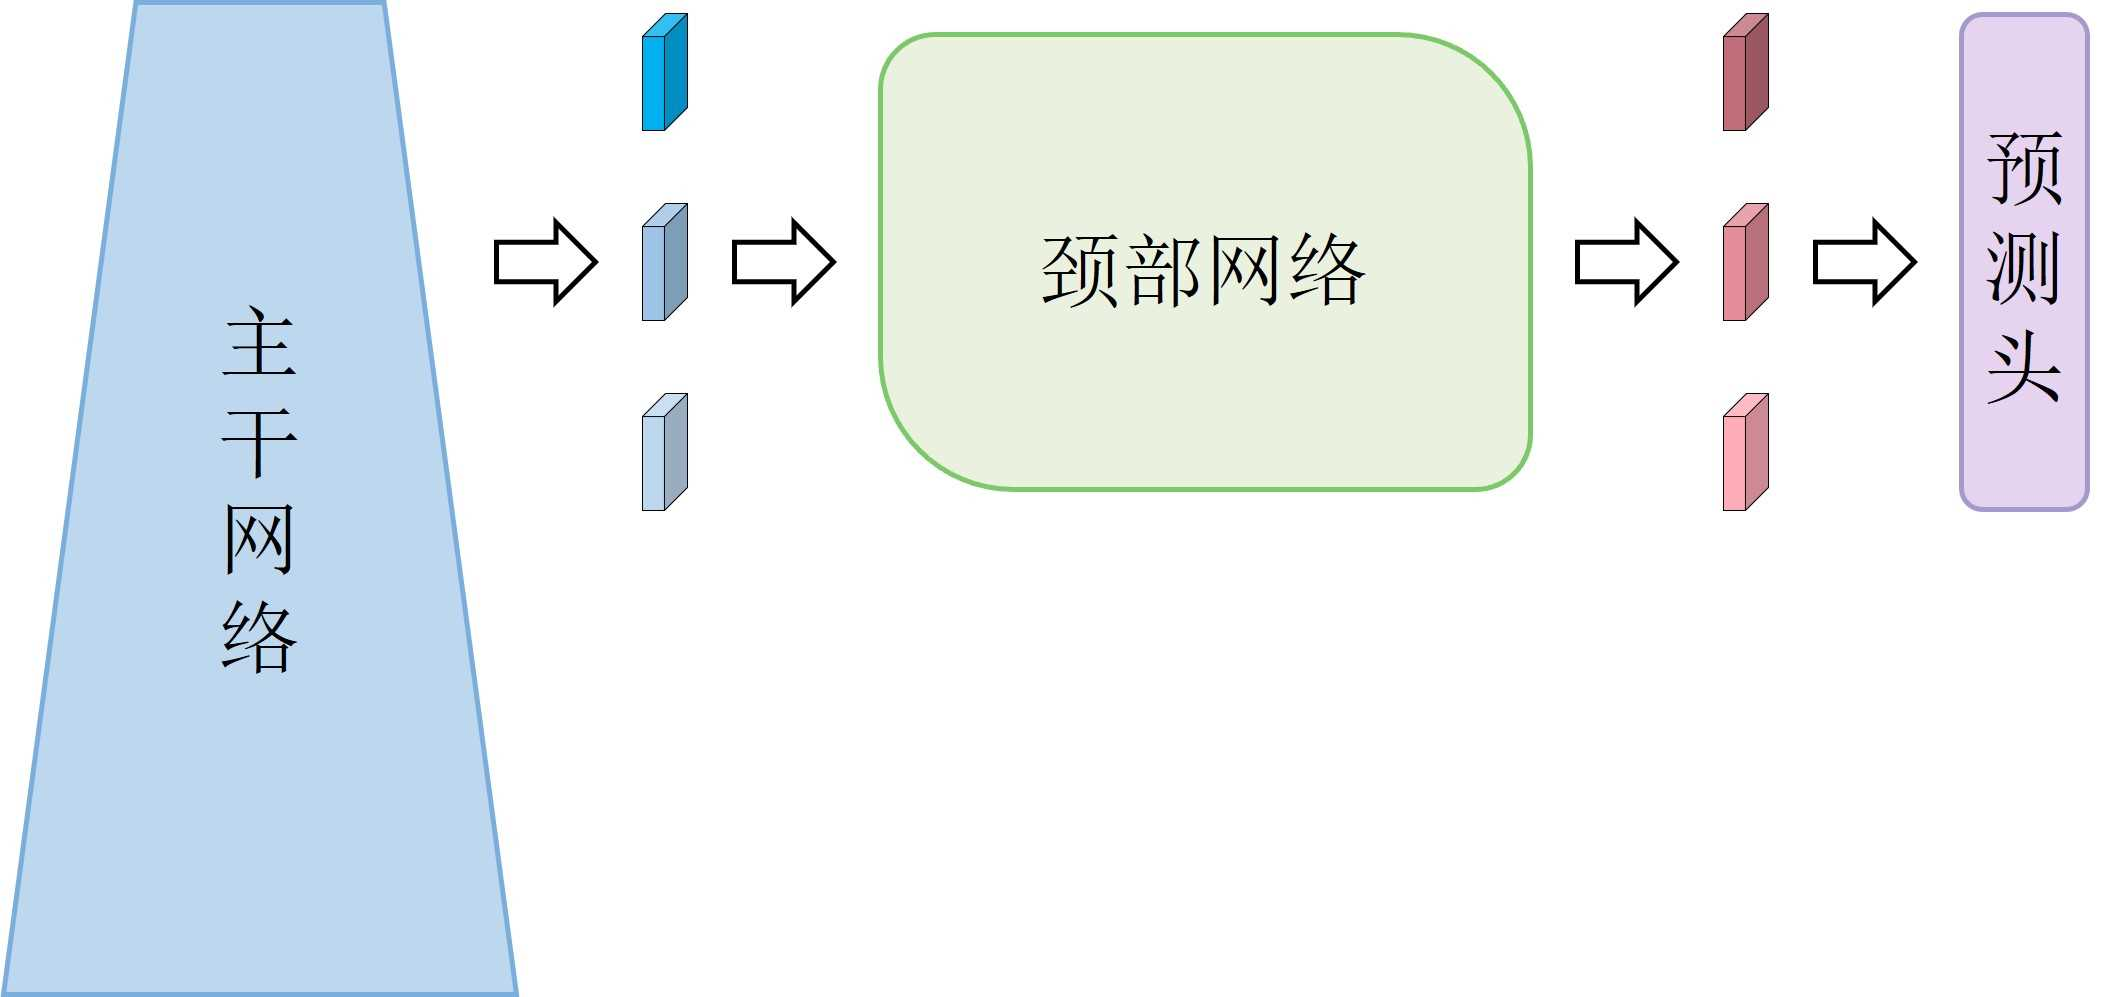
\includegraphics[width=0.8\textwidth]{figures/chap02_yolo.jpg}
  \caption{YOLO整体结构示意图}
  \label{fig:chap02_yolo}
\end{figure}

YOLO\cite{redmon2016you}(2016)是一阶段检测器中非常流行且影响深远的一种端到端的目标检测器。其核心思想是把目标检测任务转换为一个回归问题来解决。YOLO采用一个单一的神经网络结构去全图预测,如图\ref{fig:chap02_yolo},其结构可大致分为三个部分:用于特征提取的主干网络,用于特征融合的颈部网络和用于预测的头部网络。YOLO将输入图像划分为多个网格,每个网络预测多个目标的边界框和类别以及一个置信度。置信度反映了边界框包含目标的可能性。由于YOLO的设计简单直观和检测速度高效,它在现实世界中应用广泛,并且不断地在各个版本中得到改进,并确保在速度和准确度间取得更好的平衡。

YOLOv2\cite{redmon2017yolo9000}(2017)是YOLO\cite{redmon2016you}的改进模型。它在保持高速检测的特点上,通过引入批标准化、使用更高分辨率输入、增加锚框来改善边界框预测、更换主干网络以及利用多尺度训练来提高对不同尺寸目标的检测能力,从而大幅提升了检测精确度,尤其在小目标的检测上。

YOLOv3\cite{redmon2018yolov3}(2018)进一步提高了检测性能。它引入了多尺度预测来加强对小目标的识别能力,还通过加深主干网络来增加网络的特征学习能力并保持了合理的运算效率。它还采用了逻辑回归进行类别的预测,并优化了描框的机制以更好地适应不同形状的目标。整体上,YOLOv3在速度与准确度之间获得了更优的平衡。

YOLOv4\cite{bochkovskiy2020yolov4}(2020)是目标检测领域中又一重要进展,其在YOLOv3\cite{redmon2018yolov3}的基础上,综合了多项新技术来进一步提升检测准确率并且保证高速处理。该版本采用了跨阶段部分(Cross Stage Partial)\cite{wang2020cspnet}结构应用于主干网络中,引入了Mish\cite{misra2019mish}激活函数,使用了路径聚合网络(PANet)\cite{liu2018path}和空间金字塔池化(SPP)\cite{he2015spatial},增强了网络的特征提取和特征融合能力,同时包含了多种检测技术,如自适应锚框计算等等。

YOLOv5\cite{jocher2020yolov5}(2020)是YOLO系列的又一迭代,而其自身就迭代了多个版本。它采用了模块化的设计,可以选择不同大小的模型,更易于使用。YOLOv5包含了自动学习的锚框尺寸、多尺度训练、权重剪枝优化等技术,使模型既可以在资源有限的设备上运行,也能在需要高精确度的场合中保持较高性能。

YOLOX\cite{ge2021yolox}(2021)是一个新兴的目标检测架构,它在YOLOv3的基础上做了优化和改进,目标是在性能和灵活性之间取得更好的平衡。YOLOX的主要特点是它放弃了原有的锚框机制,采用了无锚框的设计,这使得网络在训练时对各种大小的目标有更好的适应能力。除此之外,YOLOX采用了解耦的头部设计,在分类和回归两个不同的任务上分开进行预测。

综上所述,一阶段目标检测器得益于算法和计算能力的提升,在目标检测任务中表现出色。它们在处理速度上显著优于二阶段检测器,满足实时处理的需求。速度的提升并未以牺牲准确率为代价,经过精心的网络设计和训练,一阶段检测器在不断地缩小与二阶段检测器的精度差距,甚至超越了它们。\textbf{因此,在PET/CT的病灶检测任务中,面对感染区域的复杂多样性,选择一阶段检测器提供了一个既快速又准确的检测策略。}

\subsection{医学影像检测算法}

在医学影像领域中,基于深度学习的检测算法已经逐步应用于现代的诊断过程之中。随着医学影像技术的发展,如MRI、CT和PET等成像技术不断进步,产生了大量的高维度和高质量的医学影像数据。这些影像含有丰富的生物医学信息,对于疾病的早期发现、诊断和治疗监测提供了重要依据。为高效、准确地解读这些复杂的数据,基于深度学习的医学影像检测算法被广泛研究和部署。

Tang等人\cite{tang2018automated}(2018)的研究提出了一种创新的架构,专门用于CT中的肺结节检测。该研究构建了一个受U-Net启发并结合3D Faster R-CNN的检测模型用于提出肺结节的候选框,还设计了一个三维卷积神经网络去降低假阳性。
Li等人\cite{li2019mvp}(2019)在神经网络设计中巧妙地融合了人类的专业知识,提出了一种具有位置感知注意力机制的多视图特征金字塔网络。该网络专门针对常见的病变检测任务,在CT的三种不同视角下,有效地利用三维医学影像信息。
Al-masni等人\cite{al2020two}(2020)提出了一种全自动、两阶段的集成深度学习框架,旨在高效地检测脑微出血。第一阶段中,YOLO被采用来识别潜在的脑微出血候选区域;随后,在第二阶段,引入了一个三维卷积网络来减少检测结果中的假阳性。
Mei等人\cite{mei2021yolo}(2021)在YOLOv4的基础上,结合各种现有的技术,如深度过参数化卷积层、卷积注意力模块和焦点损失函数,并进行了冗余的通道修剪,提出了一种更高效且实用的肺结节检测器YOLO-lung。
Lee等人\cite{lee2021dual}(2021)提出了一个创新的头颈部肿瘤分割框架。此框架采用了U形结构,设计了一种具有双分支和交叉注意力模块的编码器以及一个解码器。此外,模型集成的应用进一步强化了框架的分割性能。
Wang等人\cite{wang2022maff}(2022)提出了一种创新的多尺度自适应注意力特征融合网络,专注于PET/CT中的胰腺病变检测。该网络的核心创新体现在基于多模态的双特征提取网络和特征融合网络,以获得丰富的多尺度特征的同时让语义信息更加集中,提高了检测的精确性。
Huang等人\cite{huang2022isa}(2022)利用深度学习技术,提出了一种融合了PET高敏感度和CT精细解剖信息的创新性目标分割方法,如图\ref{fig:chap02_isanet}所示。此方法在编码阶段采用双模态的输入策略,并在解码阶段对不同模态信息进行特征融合,最大化地挖掘PET和CT各自的优势。这一方法可以有效地提高肿瘤分割性能。

\begin{figure}[htbp]
  \centering
  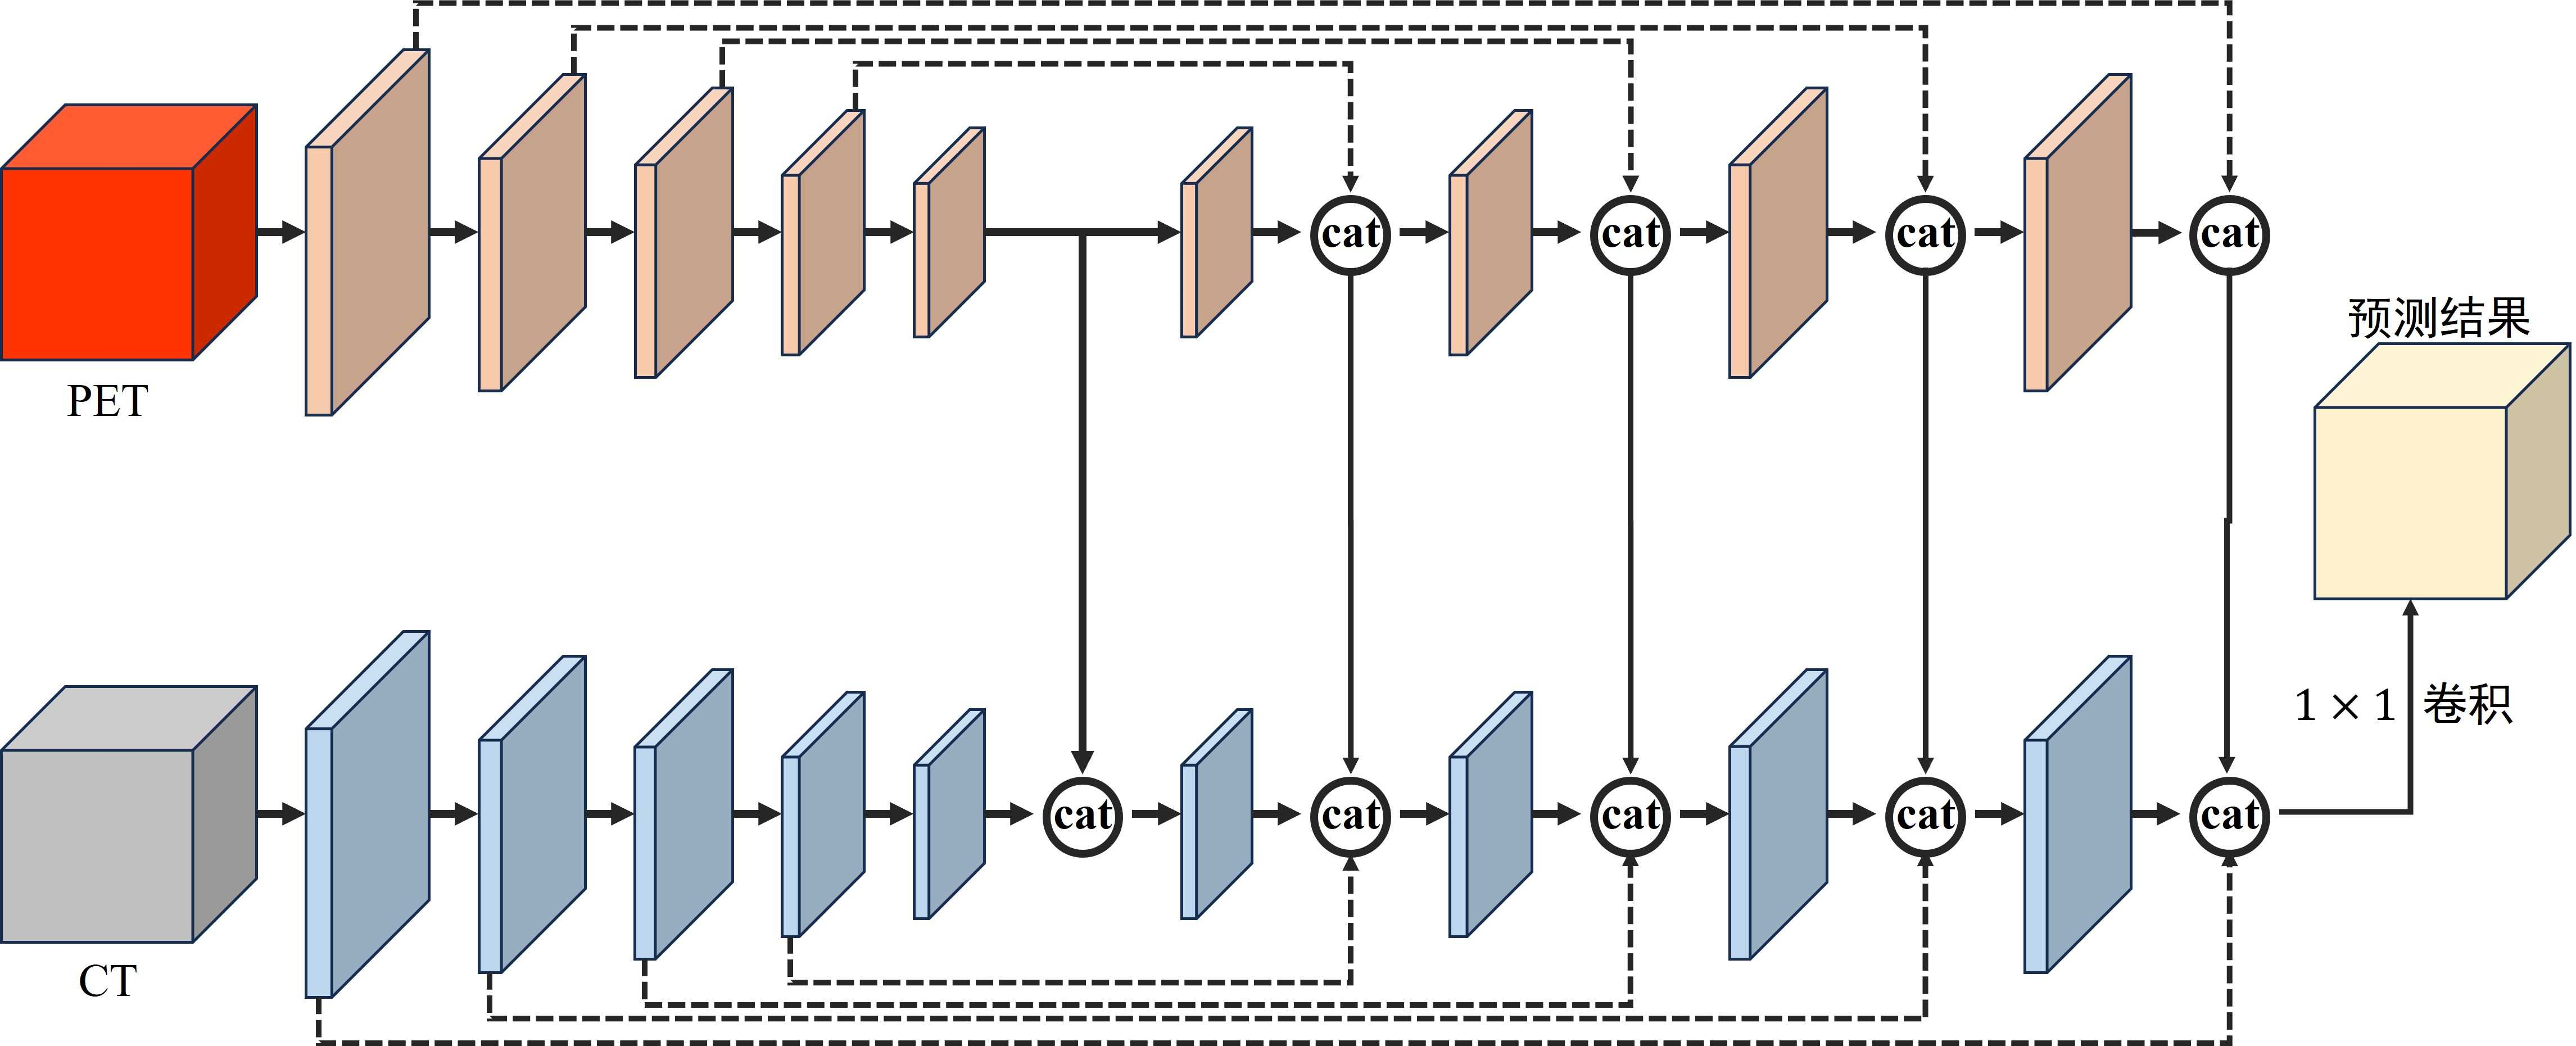
\includegraphics[width=\textwidth]{figures/chap02_isanet.jpg}
  \caption{融合PET和CT的目标分割方法}
  \label{fig:chap02_isanet}
\end{figure}

\textbf{通过上述研究,可以明确认识到在PET/CT中定位骨折相关感染的任务需要充分利用PET与CT两种不同模态提供的信息。整合和发挥两者的独特优势至关重要。因此,探讨一个双分支网络架构是一个非常值得考虑的方向。同时,还需面对PET/CT中高摄取区域所带来的干扰问题,并采用创新性的实用方法予以解决。借鉴以往研究中有效的技术方案,并结合本研究任务的具体特性,提高定位准确性是本研究努力的核心目标。}

\section{本章小结}

本章首先回顾了分类任务的核心流程及其发展变化。继而,着重解析了CNN、ViT和RNN的基础理论和关键特性,并针对本研究所涉及的分类任务,探讨了这些模型的适用性。同时,本章亦涵盖了近期医学影像领域分类研究的进展,并详细审视了这些进展对于本项研究所具有的借鉴意义。此外,特别强调了深度学习领域中检测算法的研究,梳理与总结了当下普遍应用的网络架构的发展脉络,在医学影像检测领域的最新研究动态,并从中归纳出适于本研究检测任务的方法。